% =============================================================================
% FDIC Bank Research Conference — 20-minute presentation
% Depositor Discipline in Community Banking: Evidence from the CECL
% Information Shock
%
% Slide figures: slides/figures/ (built by
%   code/result-generation/slide_figs_20260811.R; v4 histogram insets and
%   capital-quartile bars by slide_figs_v4_20260915.R)
% Reused paper figures: ../latex/figures/
% Compile: pdflatex -output-directory=build main.tex  (run twice, from slides/)
% =============================================================================
\documentclass[aspectratio=169,10pt]{beamer}

\usetheme[progressbar=frametitle,block=fill]{metropolis}
\usepackage{tikz}
\usetikzlibrary{arrows.meta,positioning,shapes.misc,fit,tikzmark}
\usepackage{booktabs}
\usepackage{colortbl}

\graphicspath{{figures/}{../latex/figures/}}

% ---- palette (matches figure palette in code/_common.R) ---------------------
\definecolor{pblue}{HTML}{1F4E79}
\definecolor{pgold}{HTML}{C9A000}
\definecolor{pgolddark}{HTML}{8A6D00}
\definecolor{pred}{HTML}{C0392B}
\definecolor{pgray}{HTML}{7F8C8D}
\definecolor{pbg}{HTML}{FAFAFA}

\setbeamercolor{normal text}{fg=black!85,bg=white}
\setbeamercolor{frametitle}{fg=white,bg=pblue}
\setbeamercolor{progress bar}{fg=pgold,bg=pgray!30}
\setbeamercolor{alerted text}{fg=pred}
\setbeamercolor{example text}{fg=pgolddark}
\setbeamercolor{title separator}{fg=pgold}
\setbeamercolor{itemize item}{fg=pblue}
\setbeamercolor{itemize subitem}{fg=pblue}
\setbeamercolor{button}{bg=pgray!20,fg=pblue}
\setbeamercolor{block title}{bg=pblue,fg=white}
\setbeamercolor{block body}{bg=pblue!7,fg=black!85}

\setbeamerfont{frametitle}{size=\large,series=\bfseries}
\setbeamertemplate{itemize item}{\textcolor{pblue}{$\blacktriangleright$}}
\setbeamertemplate{itemize subitem}{\textcolor{pgray}{--}}

% grey secondary caption line under the claim title
\newcommand{\spec}[1]{{\vspace{-2mm}\textcolor{pgray}{\footnotesize #1}\par\vspace{1mm}}}
% bottom takeaway bar
\newcommand{\takeaway}[1]{%
  \vfill
  {\centering\colorbox{pblue!8}{\parbox{0.94\textwidth}{\centering
    \textcolor{pblue}{$\Rightarrow$ \textbf{#1}}}}\par}}
% small grey inline citation
\newcommand{\gcite}[1]{{\scriptsize\textcolor{pgray}{#1}}}
% appendix pill
\newcommand{\pill}[2]{\hyperlink{#1}{\beamergotobutton{#2}}}

\title{Depositor Discipline in Community Banking}
\subtitle{Evidence from the CECL Information Shock}
\author{Dimuthu Ratnadiwakara\\{\small Federal Reserve Bank of Richmond}}
\date{{\small 25th FDIC Bank Research Conference}\\[2mm]
  {\tiny The views expressed are those of the author and do not reflect those
  of the Federal Reserve Bank of Richmond or the Federal Reserve System.}}

\begin{document}

\maketitle

% =============================================================================
\begin{frame}{Do uninsured depositors actually discipline banks?}
  \spec{Theory says they should; causal evidence has been elusive}
  \begin{itemize}
    \item<1-> Monitoring by uninsured claimants is the core private check on bank
      risk-taking \gcite{Calomiris--Kahn '91; Diamond--Rajan '01}
    \item<1-> In the data, riskier banks pay higher rates and hold fewer
      uninsured deposits, consistent with depositors pulling maturing claims
      when a bank's risk rises
      \gcite{Park--Peristiani '98; Martinez Peria--Schmukler '01;
      Goldberg--Hudgins '02}
  \end{itemize}
  \vspace{-1mm}
  {\centering\colorbox{pgold!18}{\parbox{0.94\textwidth}{\centering
    But is that correlation \textbf{discipline} (depositors reacting to news
    about risk) or \textbf{equilibrium sorting} (risky banks and yield-chasing
    depositors matching)?}}\par}
  \vspace{-1mm}
  \begin{itemize}
    \item<1-> \textbf{Policy relevance:} Main Street Depositor Protection
      Act would insure \$10M per \emph{business} account; reciprocal networks,
      sweeps, and brokers already convert uninsured money into insured money
      \gcite{Kim--Kundu--Purnanandam '24; Huberdeau-Reid--Pennacchi '25}
  \end{itemize}
  \takeaway{Needed: a shock to \emph{information} about bank risk that is
    unrelated to concurrent bank fundamentals}
\end{frame}

% =============================================================================
\begin{frame}{Why the causal evidence has been elusive: three problems}
  \begin{itemize}
    \item \textbf{Simultaneity.} A bank's risk profile, deposit mix, and
      depositor behavior co-evolve. Regressions of flows on risk measures
      capture sorting, not a disciplinary response
    \item \textbf{Accounting opacity.} Banks could delay loss recognition and
      understate risk in disclosures, so measured
      risk was partly a reporting choice
      \gcite{Beatty--Liao '11; Bushman--Williams '15}
    \item \textbf{Aggregate stress.} Episodes with the most variation in bank
      distress are also the episodes with expanded guarantees, system-wide
      shocks, and the highest liquidity needs of depositors themselves. All
      three mute or contaminate the depositor response
      \gcite{Berger--Turk-Ariss '15; Bennett--Hwa--Kwast '15}
  \end{itemize}
  \takeaway{The mandatory CECL accounting standard adoption in 2023 helps me address these
    endogeneity concerns}
\end{frame}

% =============================================================================
\begin{frame}{What is CECL? Lifetime expected losses replace incurred losses}
  \spec{ASU 2016-13 (FASB 2016), codified in ASC 326. The largest change to bank loan accounting in decades}
  \begin{columns}[T]
    \begin{column}{0.48\textwidth}
      {\centering\colorbox{pgray!15}{\parbox{0.95\linewidth}{\centering
        \textbf{Before: incurred loss (ILM)}\\[1mm]
        \footnotesize recognize a loss only when \emph{probable and
        estimable} $\Rightarrow$ provisions lag defaults, disclosures
        understate credit risk}}\par}
    \end{column}
    \begin{column}{0.48\textwidth}
      {\centering\colorbox{pblue!8}{\parbox{0.95\linewidth}{\centering
        \textbf{After: expected loss (CECL)}\\[1mm]
        \footnotesize reserve for \emph{lifetime} expected credit losses at
        origination and every reporting date $\Rightarrow$ credit risk forced
        into a reported number}}\par}
    \end{column}
  \end{columns}
  \vspace{2mm}
  At transition, the entire existing loan book is re-reserved on a single day (2023Q1):
  \[
    \Delta_i \;=\; \mathrm{ALLL}^{\mathrm{CECL}}_{i,\,t^*}
      \;-\; \mathrm{ALLL}^{\mathrm{ILM}}_{i,\,t^*-1}
    \qquad \text{\footnotesize (one-time charge to retained earnings,
      no cash flow)}
  \]
  \vspace{-2mm}
  \[
    \text{Treatment:}\qquad
    \texttt{CECL Adj}_i \;=\; \frac{\Delta_i}{\mathrm{Equity}_{i,\,t^*-1}}
      \times 100
  \]
  \takeaway{$\Delta_i$ reflects the composition and seasoning of loans made
    years earlier, not deposit-market conditions in 2023}
\end{frame}

% =============================================================================
\begin{frame}{The experiment: a mandatory disclosure with a predetermined size}
  \spec{CECL Day-One adjustment = one-time charge to retained earnings, fixed by past underwriting}
  \begin{center}
  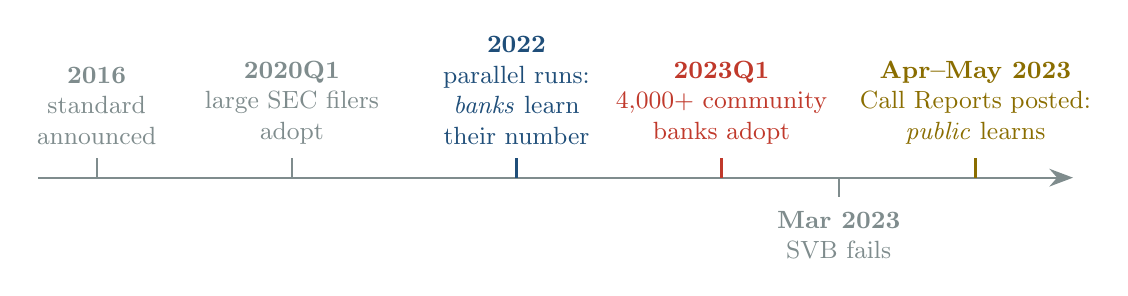
\begin{tikzpicture}[x=1.24cm, every node/.style={font=\small}]
    % axis
    \draw[-{Stealth[length=3mm]}, thick, pgray] (0,0) -- (10.6,0);
    % events
    \foreach \x/\lab/\col in {0.6/{\textbf{2016}\\standard\\announced}/pgray,
      2.6/{\textbf{2020Q1}\\large SEC filers\\adopt}/pgray}{
      \draw[\col, thick] (\x,0) -- (\x,0.25);
      \node[above, align=center, text=\col] at (\x,0.3) {\lab};
    }
    \draw[pblue, very thick] (4.9,0) -- (4.9,0.25);
    \node[above, align=center, text=pblue] at (4.9,0.3)
      {\textbf{2022}\\parallel runs:\\\emph{banks} learn\\their number};
    \draw[pred, very thick] (7.0,0) -- (7.0,0.25);
    \node[above, align=center, text=pred] at (7.0,0.3)
      {\textbf{2023Q1}\\4{,}000+ community\\banks adopt};
    \draw[pgray, thick] (8.2,0) -- (8.2,-0.25);
    \node[below, align=center, text=pgray] at (8.2,-0.3)
      {\textbf{Mar 2023}\\SVB fails};
    \draw[pgolddark, very thick] (9.6,0) -- (9.6,0.25);
    \node[above, align=center, text=pgolddark] at (9.6,0.3)
      {\textbf{Apr--May 2023}\\Call Reports posted:\\\emph{public} learns};
  \end{tikzpicture}
  \end{center}
  \vspace{1mm}
  \begin{itemize}
    \item Pure accounting event: no cash flow, no change in loan risk. Only
      \textbf{news} about lifetime expected losses already embedded in the book
    \item Everyone knew \emph{when} since 2016. Nobody outside the bank
      knew \emph{how much} until the Call Report was posted
    \item Timing wedge: banks knew their number in 2022, the public only in
      April--May 2023
  \end{itemize}
\end{frame}

% =============================================================================
\begin{frame}[label=ftreat]{Treatment: the disclosed charge, scaled by equity}
  \spec{4{,}320 community banks ($<$\$10B); charge disclosed on Schedule RI-A of the adoption-quarter Call Report}
  \begin{columns}[T]
    \begin{column}{0.62\textwidth}
      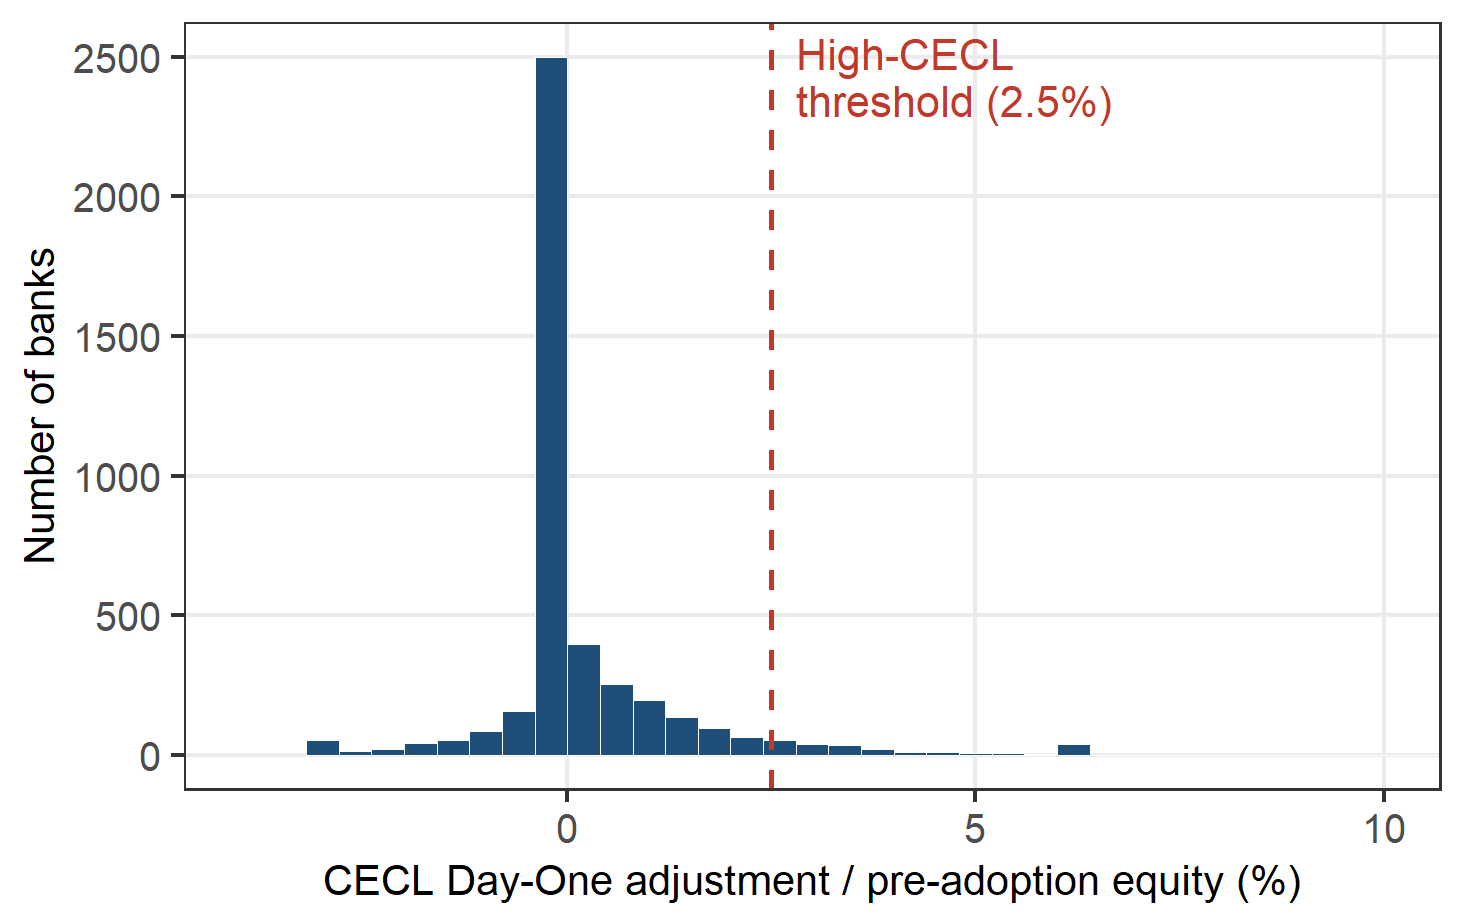
\includegraphics[width=\linewidth]{fig_s_cecl_dist.png}
    \end{column}
    \begin{column}{0.36\textwidth}
      \vspace{4mm}
      {\Large\textbf{\textcolor{pblue}{92\%}}} adopt in 2023Q1\\[2.5mm]
      {\Large\textbf{\textcolor{pblue}{$\sim$half}}} disclose a charge
        of about zero\\[2.5mm]
      {\Large\textbf{\textcolor{pred}{217}}} High-CECL banks:
        charge $\geq$ 2.5\% of equity ($\approx$95th pctile),
        mean 4\% of equity\\[3mm]
      {\centering\colorbox{pgold!18}{\parbox{0.95\linewidth}{\footnotesize
        \textbf{Charge is hard to predict:} 2022Q4 observables explain
        $\sim$1\% of its variation \pill{apppredictors}{detail}}}\par}
    \end{column}
  \end{columns}
\end{frame}

% =============================================================================
\begin{frame}{Is the CECL charge a big deal? Markets repriced it in 2020}
  \spec{Large SEC filers adopted 2020Q1, three years before community banks; monthly event studies, coefficient on charge/equity}
  \begin{columns}[T]
    \begin{column}{0.5\textwidth}
      \centering {\small Market capitalization}\\
      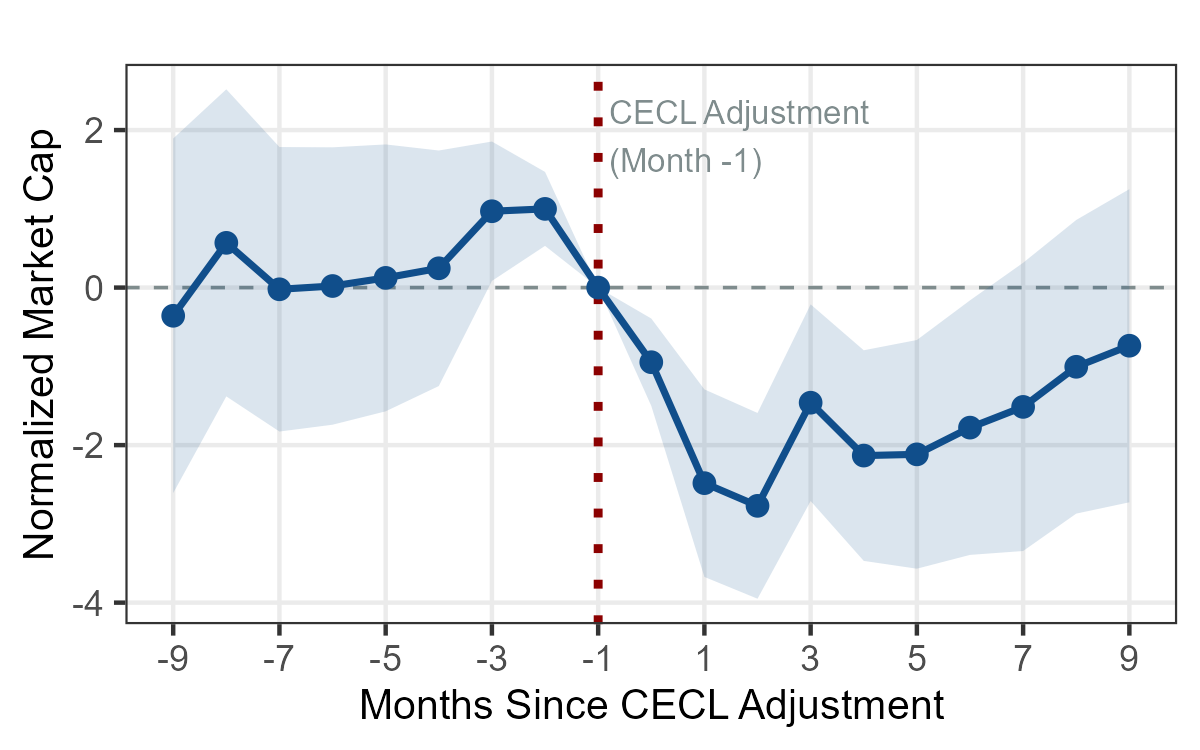
\includegraphics[width=\linewidth]{mkt_cap_large_banks_20260403.png}
    \end{column}
    \begin{column}{0.5\textwidth}
      \centering {\small 5-year CDS spread}\\
      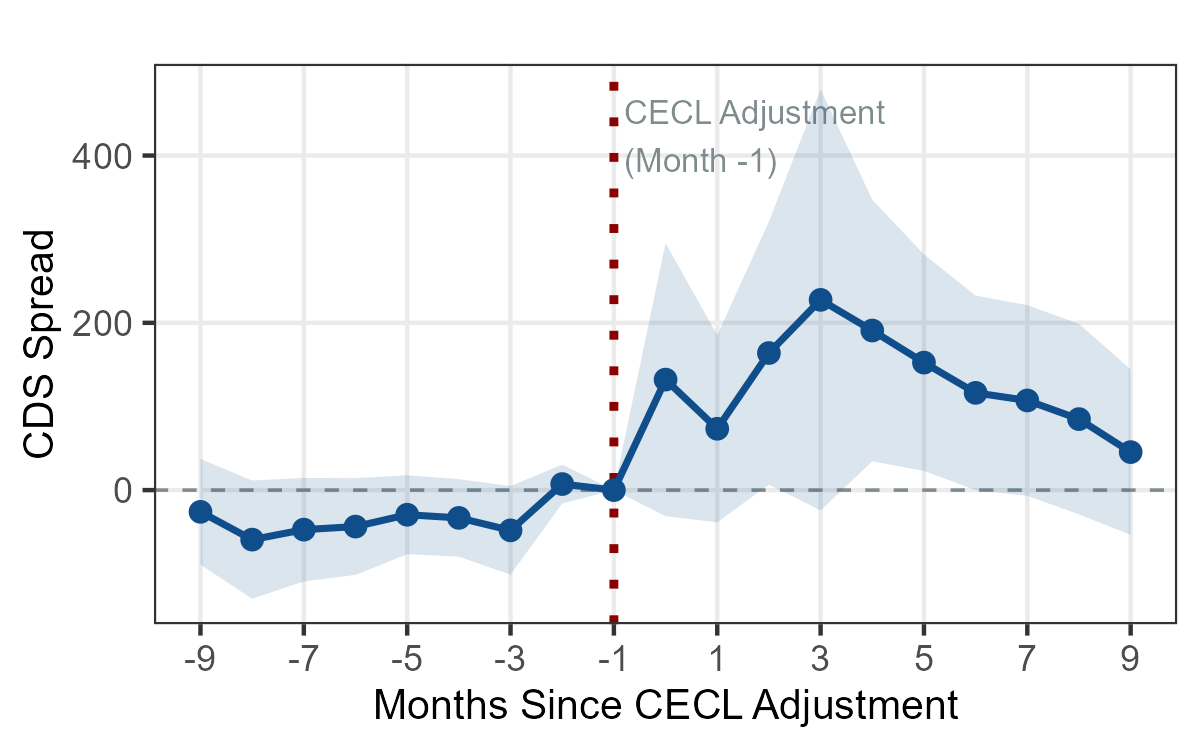
\includegraphics[width=\linewidth]{cds_spread_large_banks_20260403.png}
    \end{column}
  \end{columns}
  \takeaway{Equity falls $\sim$2.8\% per pp of charge at adoption; CDS spreads
    widen with a lag}
\end{frame}

% =============================================================================
\begin{frame}{Data: quarterly Call Reports for 4{,}320 community banks, 2016--2025}
  \spec{FFIEC 041/051, 2016Q1--2025Q4 ($\sim$97{,}000 bank-quarters); RateWatch posted rates; CRSP + Bloomberg for the 2020 cohort}
  \begin{columns}[T]
    \begin{column}{0.41\textwidth}
      \begin{itemize}
        \item Federally insured banks $<$ \$10B in assets at 2022Q4;
          median bank \$0.3B
        \item Deposit breakdowns by insurance status from Schedule RC-E;
          outcomes scaled by assets
        \item Time deposits fund \textbf{12.7\%} of assets
          (5.3 uninsured $+$ 7.4 insured)
      \end{itemize}
    \end{column}
    \begin{column}{0.57\textwidth}
      \centering
      {\scriptsize
      \setlength{\tabcolsep}{4pt}
      \begin{tabular}{lrrr}
        \toprule
        Pre-adoption means & High CECL & Low CECL & Hi$-$Lo \\
        \midrule
        CECL Adj / Equity (\%) & 3.99 & 0.08 & 3.91*** \\
        NPL / Loans (\%) & 0.60 & 0.45 & 0.15*** \\
        Equity / Assets (\%) & 8.88 & 10.34 & $-$1.46*** \\
        Ins.\ time dep.\ / Assets (\%) & 9.13 & 7.27 & 1.86*** \\
        \rowcolor{pgold!15}
        Unins.\ time dep.\ / Assets (\%) & 5.62 & 5.28 & 0.33\phantom{***} \\
        \bottomrule
      \end{tabular}}
      \vspace{1.5mm}

      {\footnotesize High-CECL banks: weaker loan quality, thinner capital.
      But \textbf{balanced on the primary outcome} (bank FE absorb the
      levels)}
    \end{column}
  \end{columns}
\end{frame}

% =============================================================================
\begin{frame}{Raw group means: uninsured and insured time deposits around adoption}
  \spec{Group means, pp of assets; 206 High-CECL vs 2{,}265 near-zero banks; no controls or FE}
  \centering
  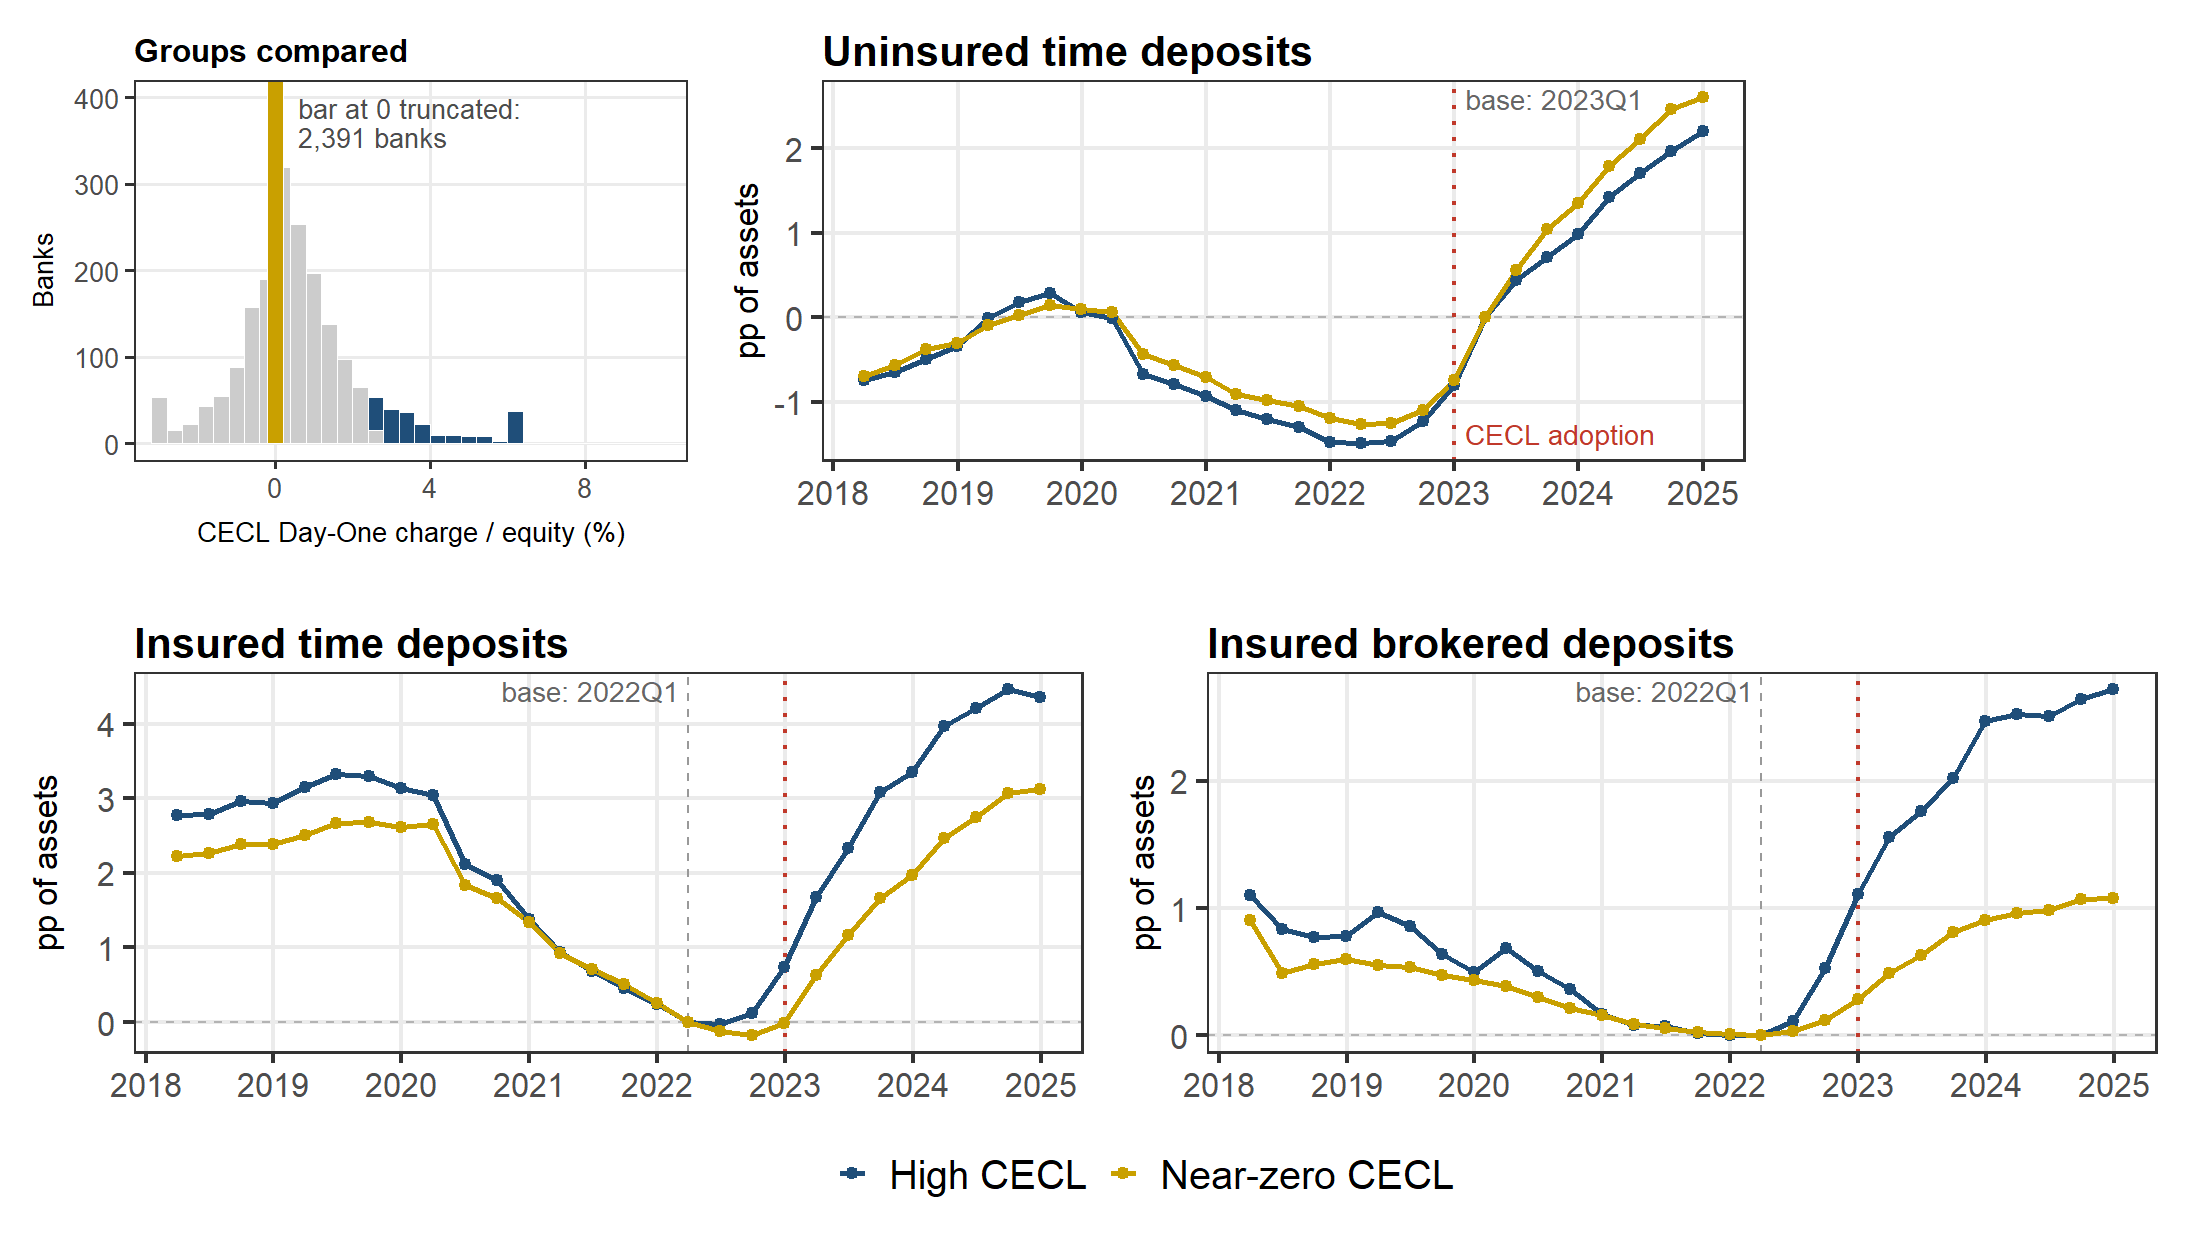
\includegraphics[width=\linewidth,height=0.84\textheight,keepaspectratio]{fig_s_motiv_panels.png}
\end{frame}

% =============================================================================
\begin{frame}[label=fstrategy]{Empirical strategy}
  \spec{Bank + calendar-quarter FE; SEs clustered by bank; controls: lagged log assets, equity/assets, int.\ exp./assets}
  \begin{block}{Specification 1: level DiD \emph{across} banks
    (expected sign $\beta<0$)}
    \vspace{-2mm}
    \[
      y_{it} = \alpha_i + \gamma_t + \alert{\beta}\,\mathrm{Post}_{it}\times
        \mathrm{CECL}_i + X_{it-1}'\delta + \varepsilon_{it}
    \]
    \vspace{-6mm}

    {\scriptsize $\mathrm{CECL}_i$: continuous \texttt{CECL Adj} or High-CECL
    indicator; event studies replace $\mathrm{Post}$ with event-time dummies,
    $k=-1$ omitted. Quarter FE absorb the tightening cycle and any aggregate
    2023-stress response.}
  \end{block}
  \vspace{6mm}
  \pause
  \begin{block}{Specification 2: triple difference \emph{within}
    bank$\times$quarter (series stacked)}
    \vspace{-4mm}
    \begin{align*}
      y_{idt} = \alpha_{it}
        &+ \beta_2\,\mathrm{Post}_t\times\mathrm{Unins}_d
         + \beta_3\,\mathrm{CECL}_i\times\mathrm{Unins}_d \\[-1mm]
        &+ \alert{\beta_4}\,\mathrm{CECL}_i\times\mathrm{Post}_t\times
          \mathrm{Unins}_d + \varepsilon_{idt}
    \end{align*}
    \vspace{-6mm}

    {\scriptsize $\alpha_{it}$ absorbs \emph{every} bank-level shock in every
    quarter: funding demand, stress exposure, liability strategy. $\beta_4$
    is identified only from the within-bank uninsured-vs-insured differential.}
  \end{block}
\end{frame}

% =============================================================================
\begin{frame}{Uninsured time deposits are flat for ten quarters\dots\ then break at disclosure}
  \spec{Event study, High-CECL $\times$ event time; bank + quarter FE; 90\% CI}
  \centering
  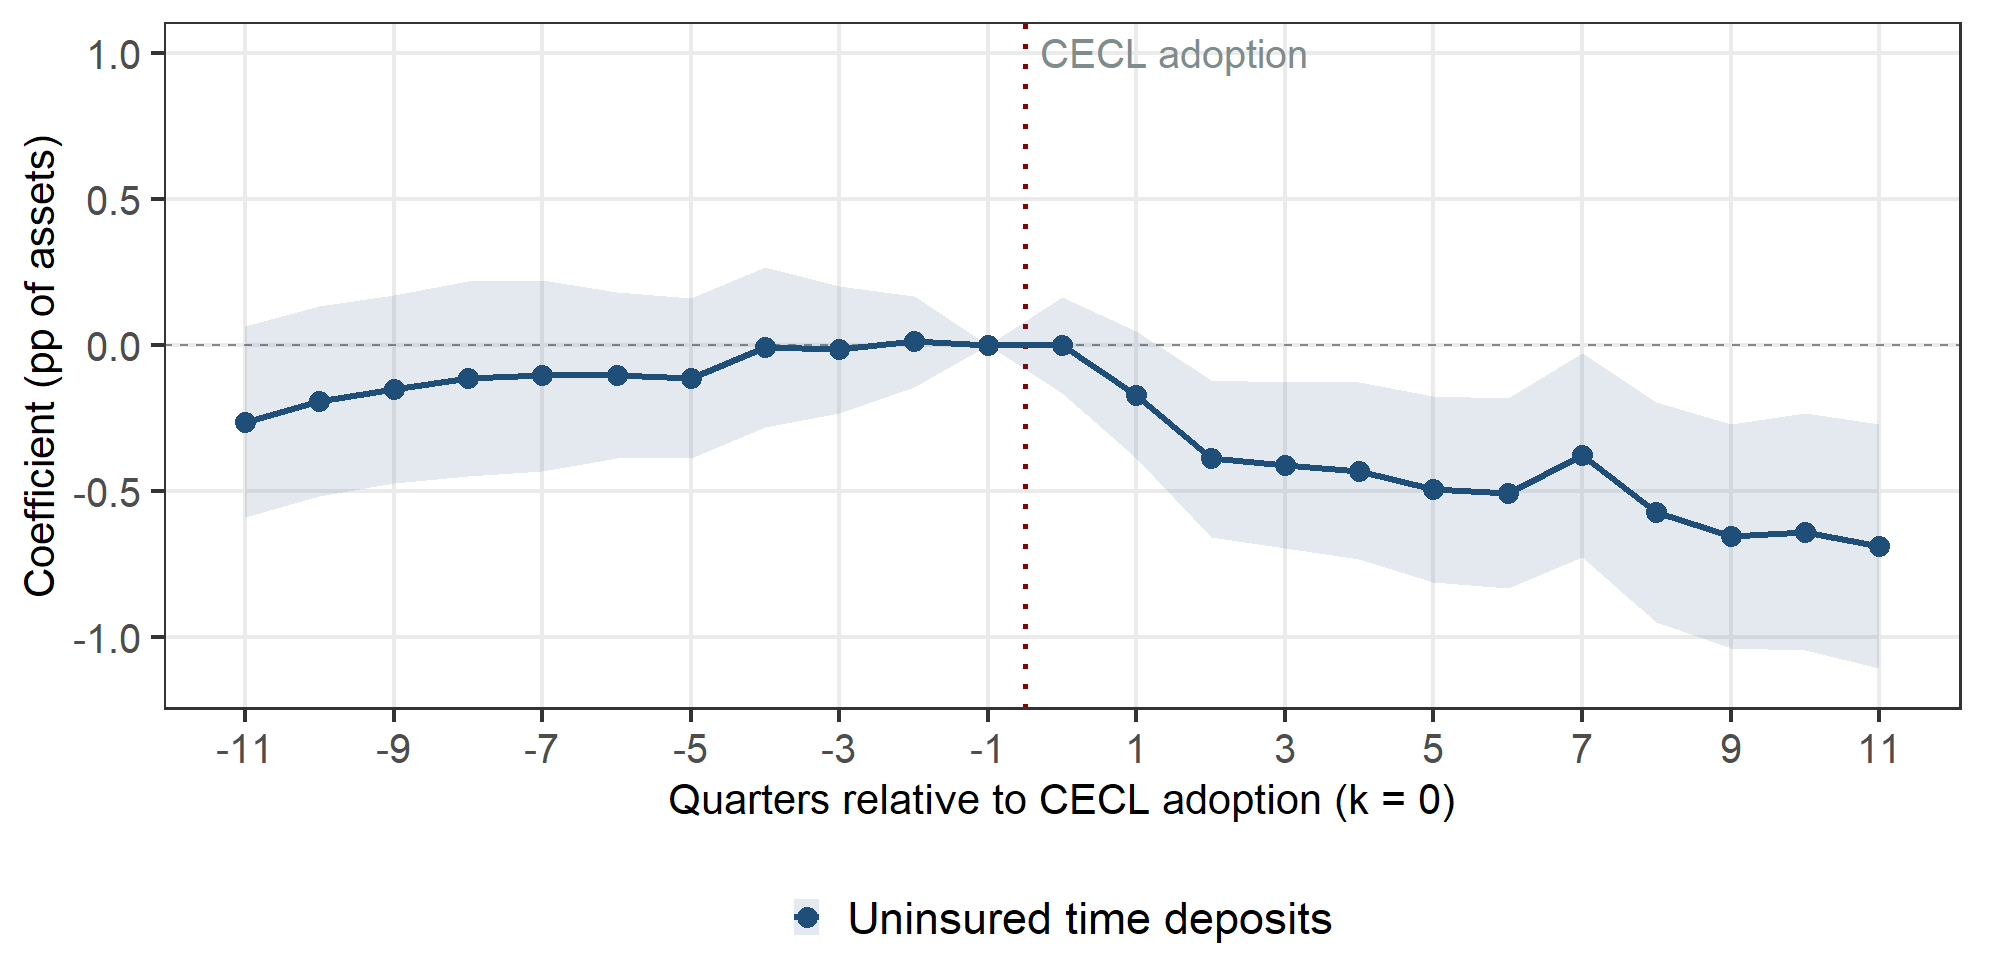
\includegraphics[width=0.92\linewidth,height=0.68\textheight,keepaspectratio]{fig_s_overlay_build1.png}
\end{frame}

\begin{frame}{\dots while insured time deposits rise}
  \spec{Same specification, insured series overlaid; identical axes}
  \centering
  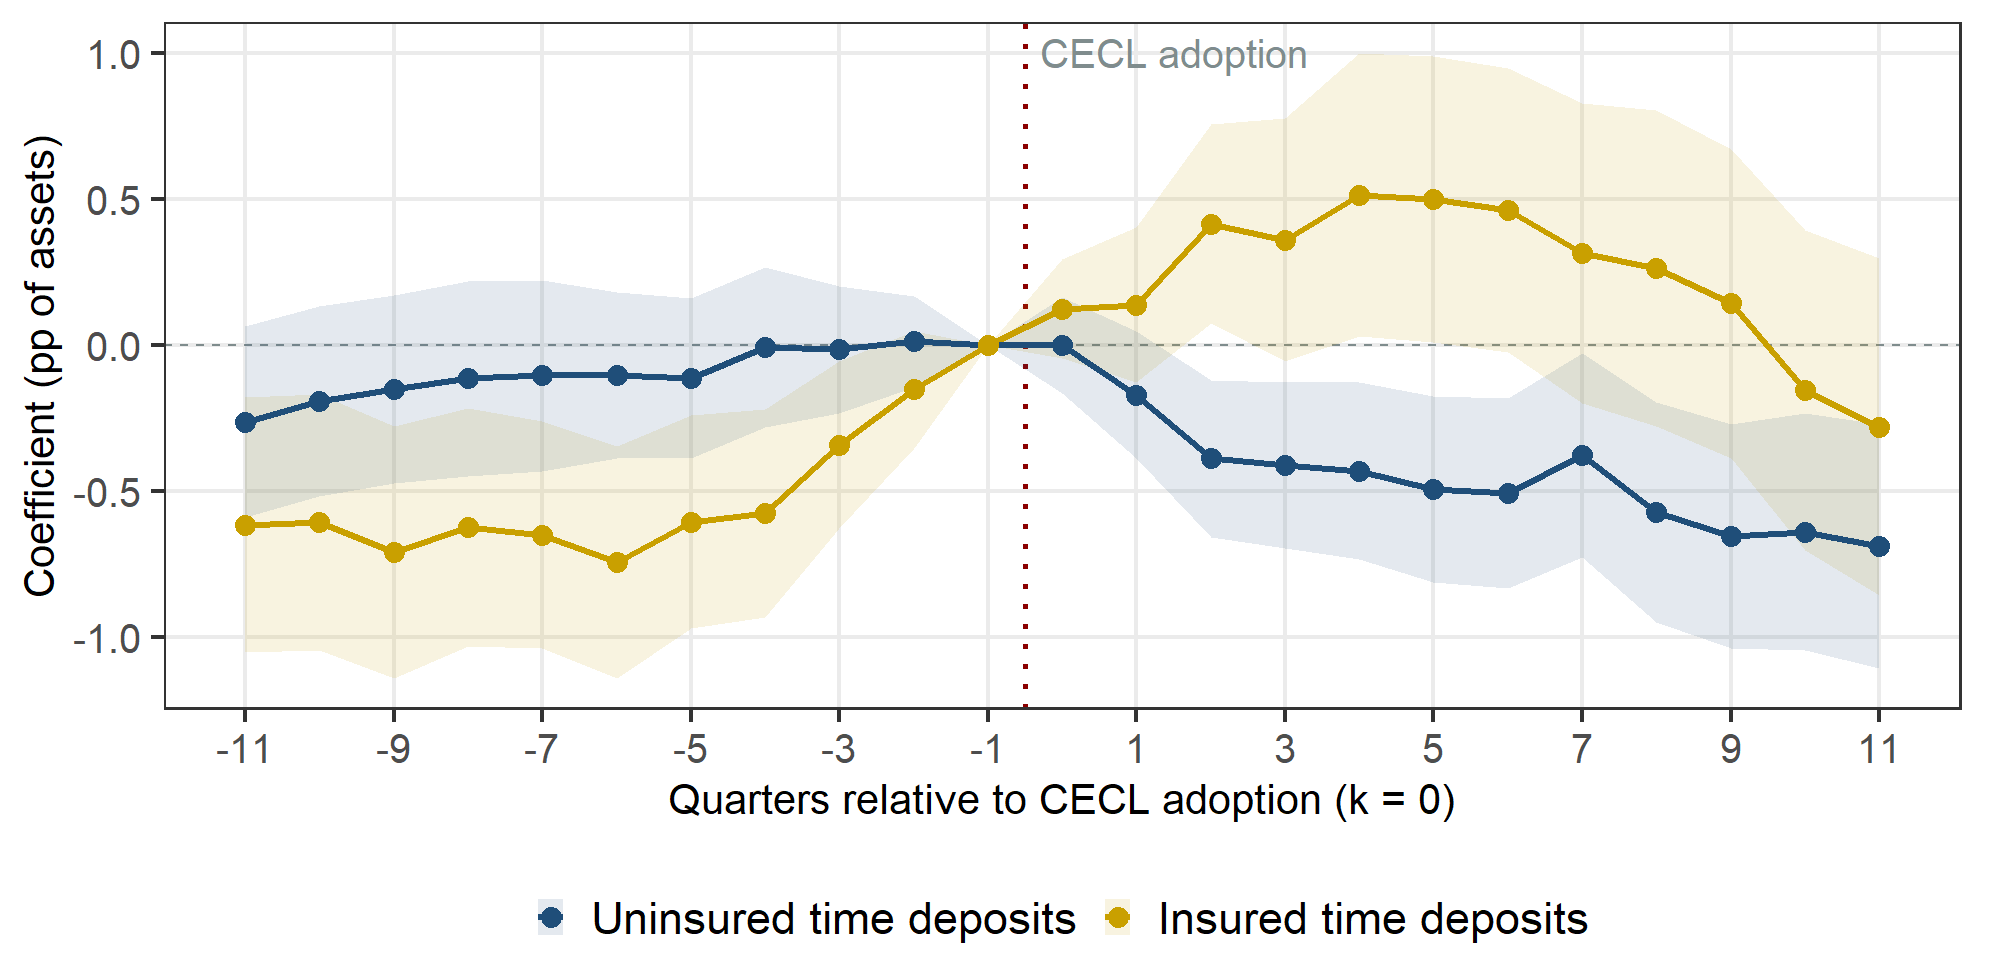
\includegraphics[width=0.92\linewidth,height=0.68\textheight,keepaspectratio]{fig_s_overlay_build2.png}
\end{frame}

% =============================================================================
\begin{frame}[label=fmag]{Baseline estimates: uninsured time deposits fall, insured time deposits rise}
  \spec{Each row is a separate regression. Coefficients in pp of assets; bank-clustered inference; */**/*** = 10/5/1\% \quad \pill{fstrategy}{specification}}
  \vspace{-3mm}
  \begin{center}
  {\small
  \setlength{\tabcolsep}{9pt}
  \renewcommand{\arraystretch}{1.2}
  \begin{tabular}{lccc}
    \toprule
    & Unins.\ time dep. & Ins.\ time dep. & Unins.\ $-$ ins.\ gap \\
    & / assets & / assets & (composition) \\
    \midrule
    \rowcolor{pblue!8}
    \textcolor<2>{pgray}{Post $\times$ High CECL} & \tikz[baseline=(hl.base)]\node[draw=pred, very thick, rounded corners, inner sep=2.5pt] (hl) {\textcolor<2>{pgray}{$-$0.39**}}; & \textcolor<2>{pgray}{$+$0.71**} & \textcolor<2>{pgray}{$-$1.25***} \\
    \uncover<2->{Post $\times$ CECL Adj (continuous)} & \uncover<2->{$-$0.072**} & \uncover<2->{$+$0.070\phantom{**}} & \uncover<2->{$-$0.177***} \\
    \midrule
    Bank $+$ quarter FE & \checkmark & \checkmark & --- \\
    Bank $\times$ quarter FE & --- & --- & \checkmark \\
    Observations & 97{,}064 & 97{,}064 & 194{,}128 \\
    \bottomrule
  \end{tabular}}
  \end{center}
\end{frame}

% =============================================================================
\begin{frame}{Heterogeneity by deposit type and by CD maturity}
  \spec{Same specification as the table. Interaction coefficients shown graphically with 90\% CIs from here on}
  \begin{columns}[T]
    \begin{column}{0.64\textwidth}
      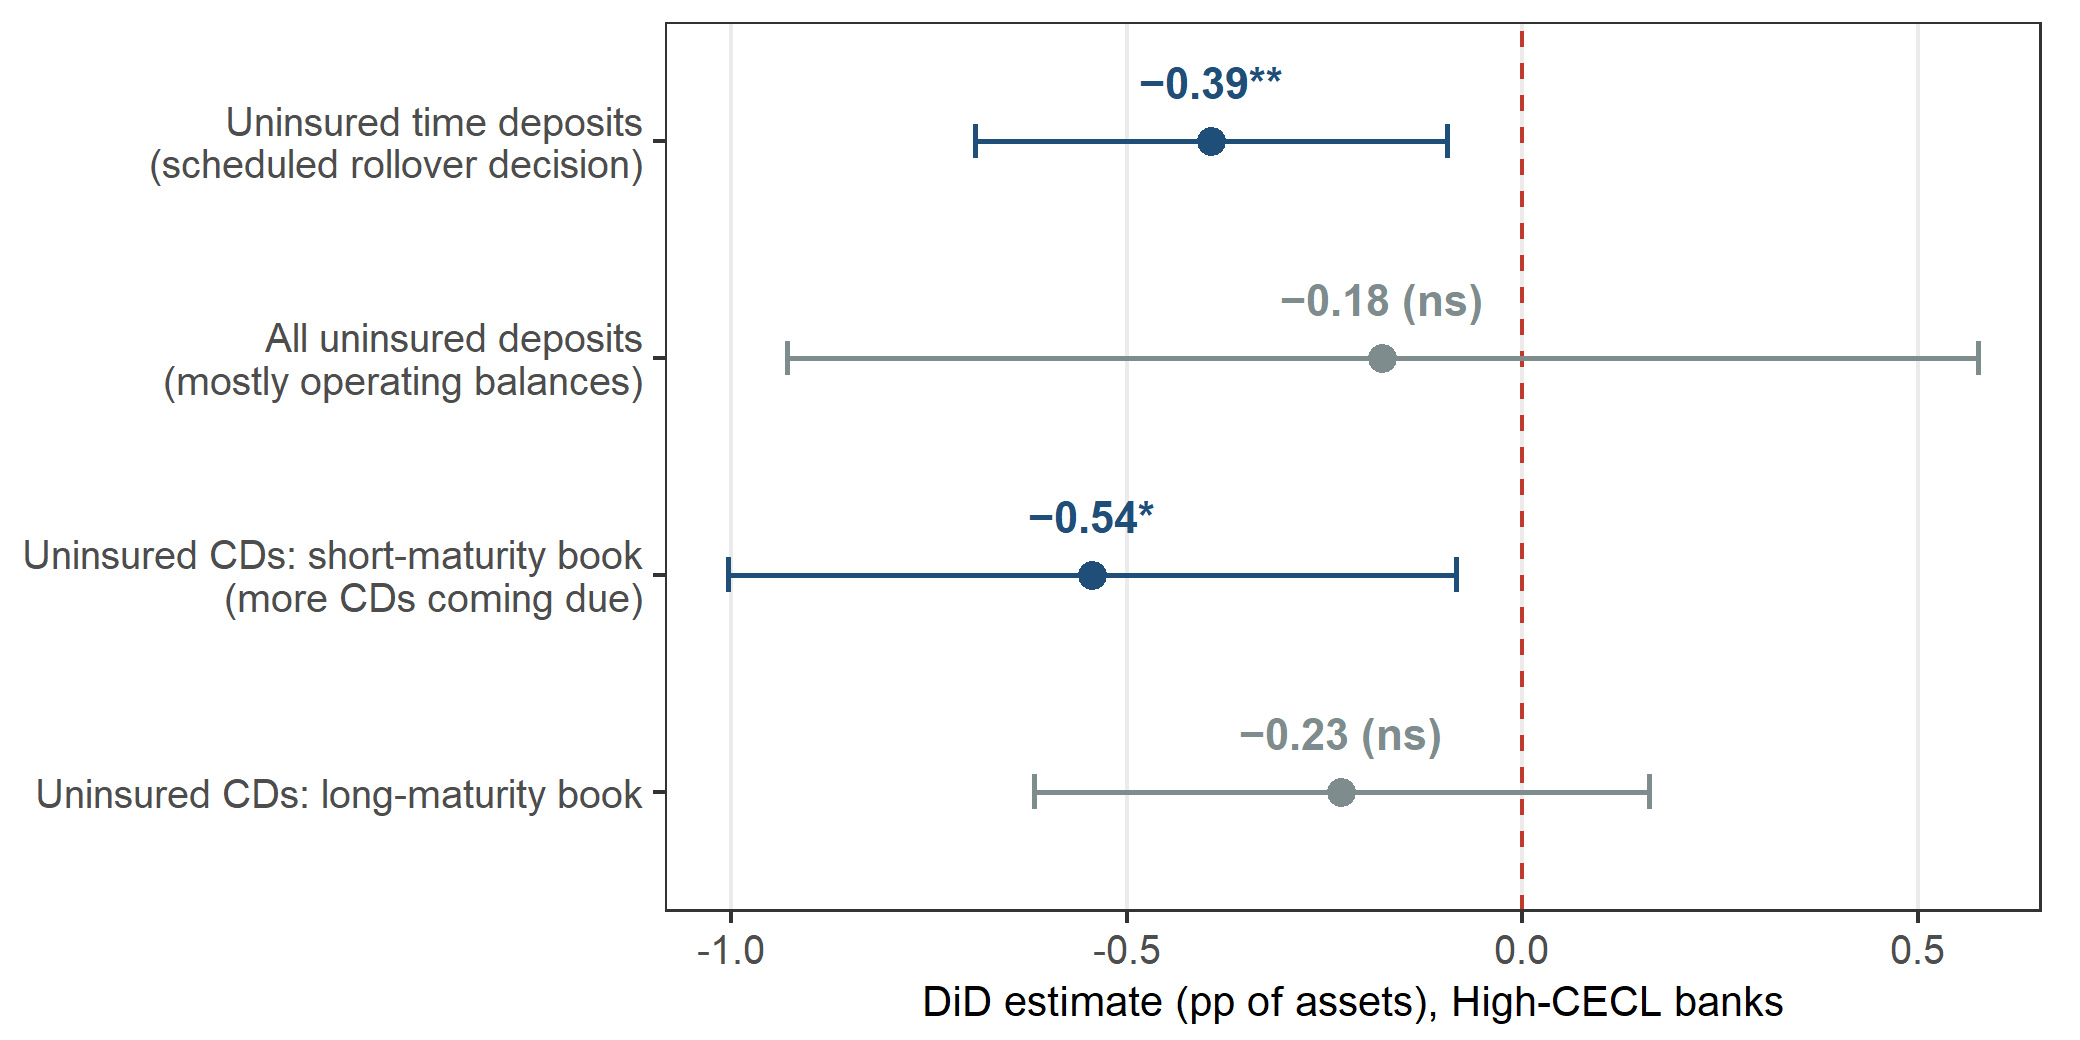
\includegraphics[width=\linewidth,height=0.62\textheight,keepaspectratio]{fig_s_coef_margin.png}
    \end{column}
    \begin{column}{0.34\textwidth}
      \vspace{6mm}
      \uncover<2->{\colorbox{pgold!18}{\parbox{0.94\linewidth}{\scriptsize\raggedright
      \textbf{Why no response in total uninsured deposits?}\\[0.8mm]
      At the median bank, balances over \$250k are 34\% of assets. Of these,
      23\% are municipal deposits, collateralized by pledged securities, and
      26\% are noninterest-bearing operating accounts, held for liquidity
      services rather than yield \gcite{d'Avernas et al.\ '23}.\\[0.8mm]
      This money has no scheduled decision point and no reason to respond to
      a credit disclosure.}}}
    \end{column}
  \end{columns}
\end{frame}

% =============================================================================
\begin{frame}[label=fcapital]{The response is concentrated at thinly capitalized banks}
  \spec{Post $\times$ High CECL on uninsured time deposits/assets, split at median 2022Q4 equity/assets (9.8\%); bank + quarter FE; 90\% CI \quad \pill{appcapital}{continuous version}}
  \centering
  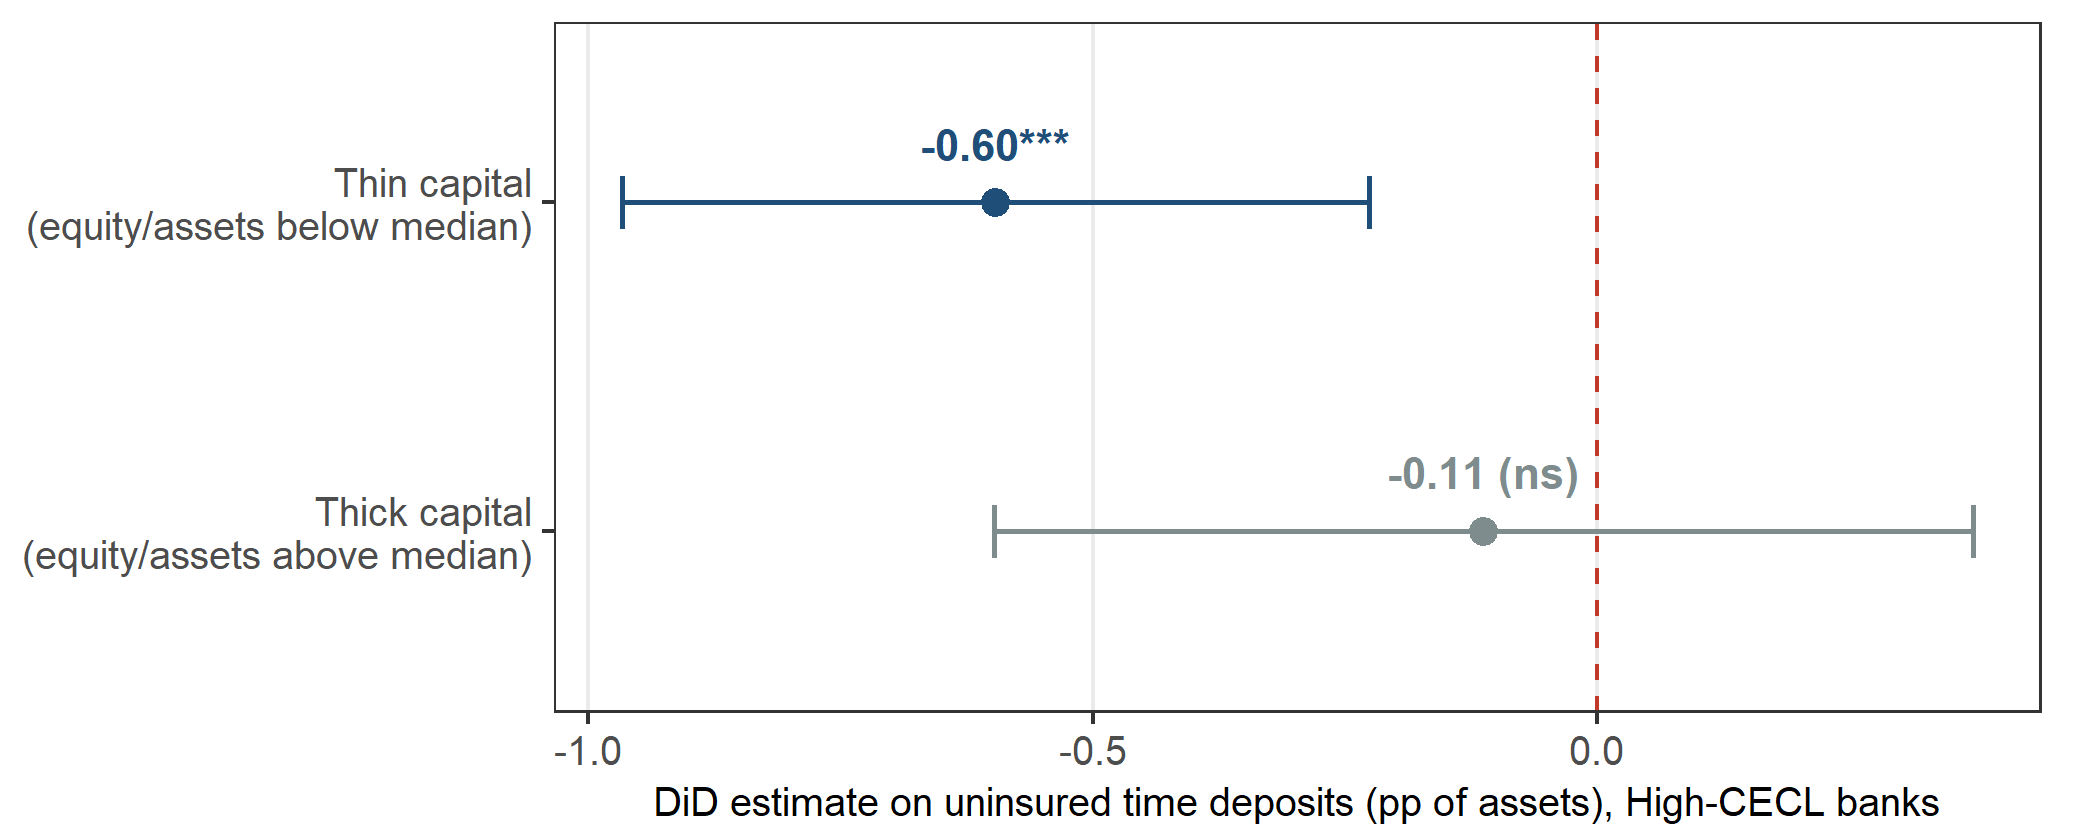
\includegraphics[width=0.76\linewidth,height=0.6\textheight,keepaspectratio]{fig_s_capital_quartiles.png}
\end{frame}

% =============================================================================
\begin{frame}[label=fcapmat]{Both margins together: thin capital \emph{and} near-term CD maturities}
  \spec{Post $\times$ High CECL on uninsured time deposits/assets, in the 2$\times$2 of 2022Q4 capital (median 9.8\%) and 2022Q4 share of uninsured CDs maturing within one year (median 76\%); bank + quarter FE; 90\% CI}
  \centering
  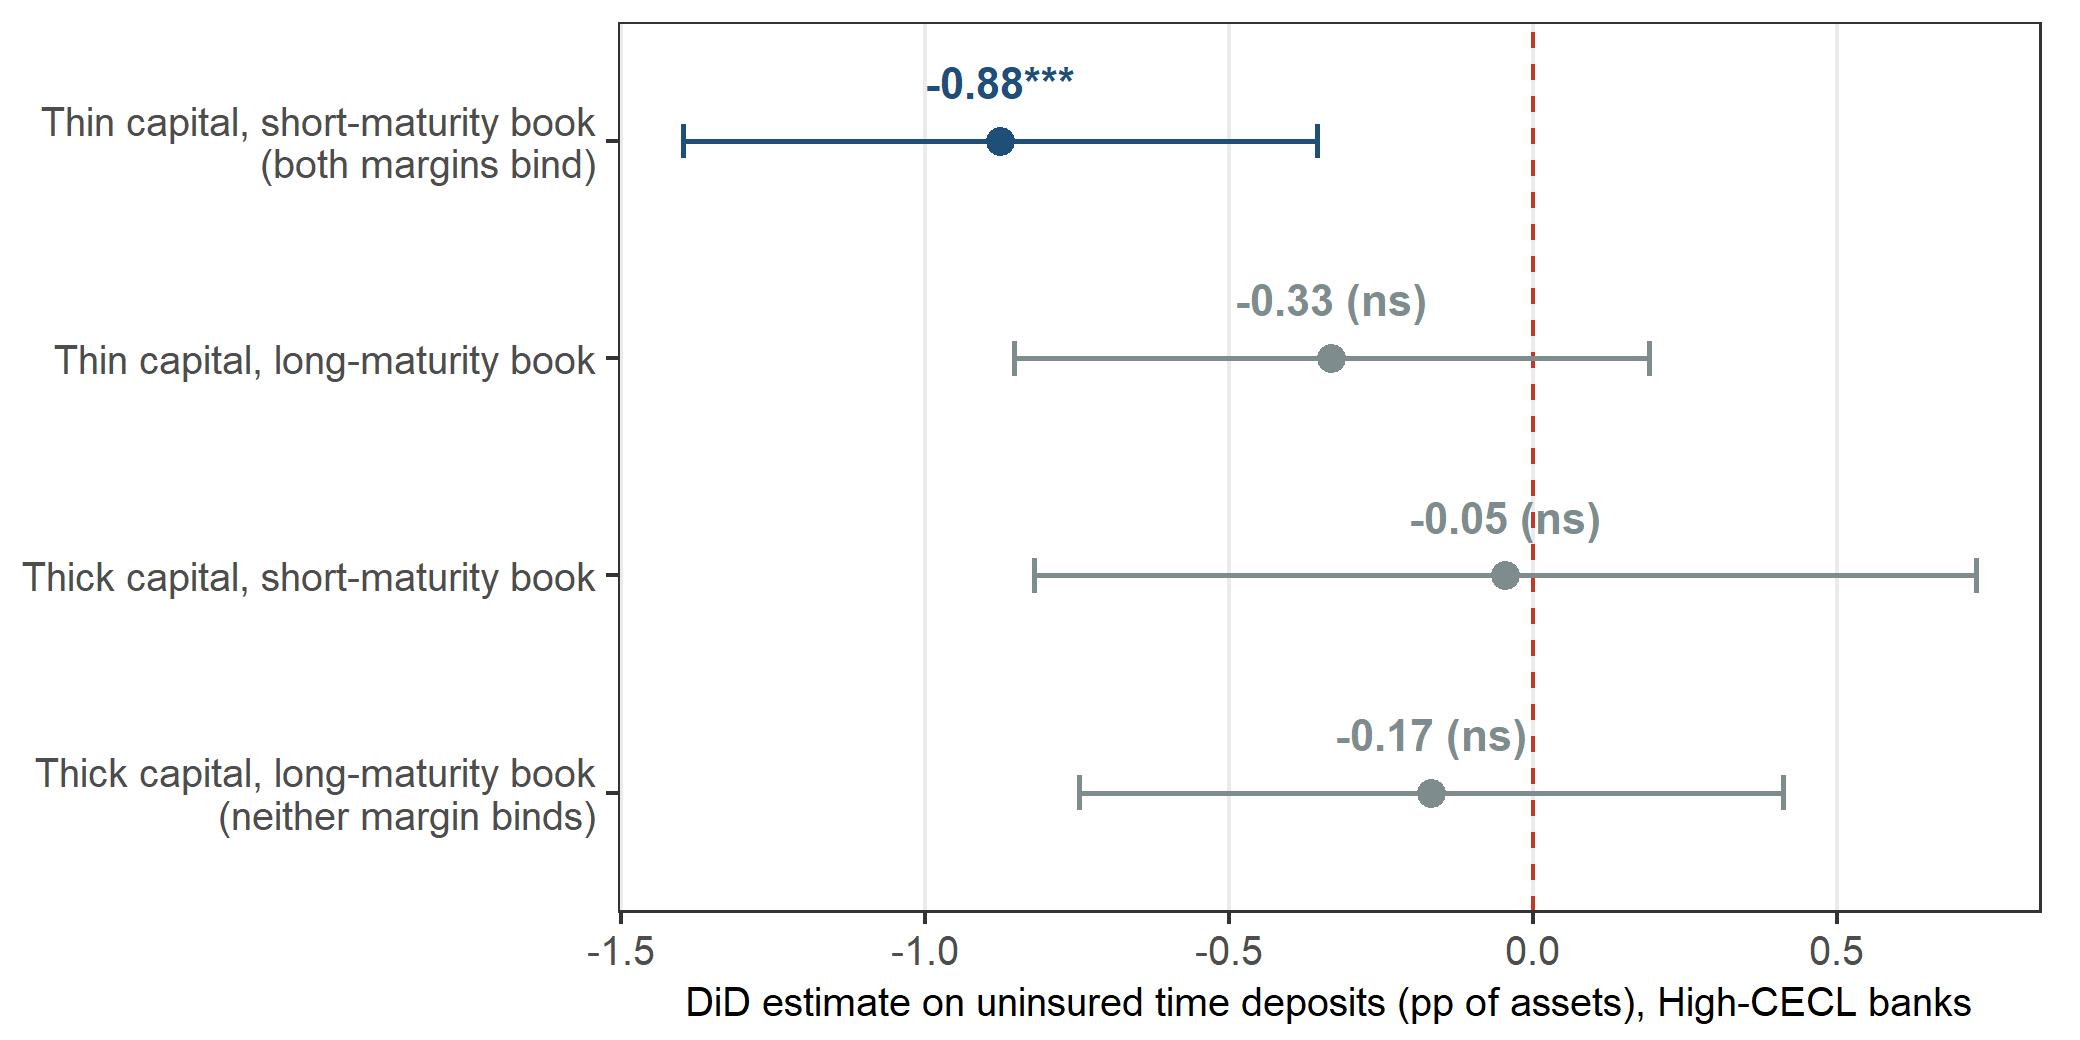
\includegraphics[width=0.76\linewidth,height=0.6\textheight,keepaspectratio]{fig_s_capital_maturity_2x2.png}
\end{frame}

% =============================================================================
\begin{frame}[label=fcapmattotal]{The same 2$\times$2 for total uninsured deposits}
  \spec{Post $\times$ High CECL on total uninsured deposits/assets (mean 35\% of assets); same cells, controls, and fixed effects as the previous slide; 90\% CI}
  \centering
  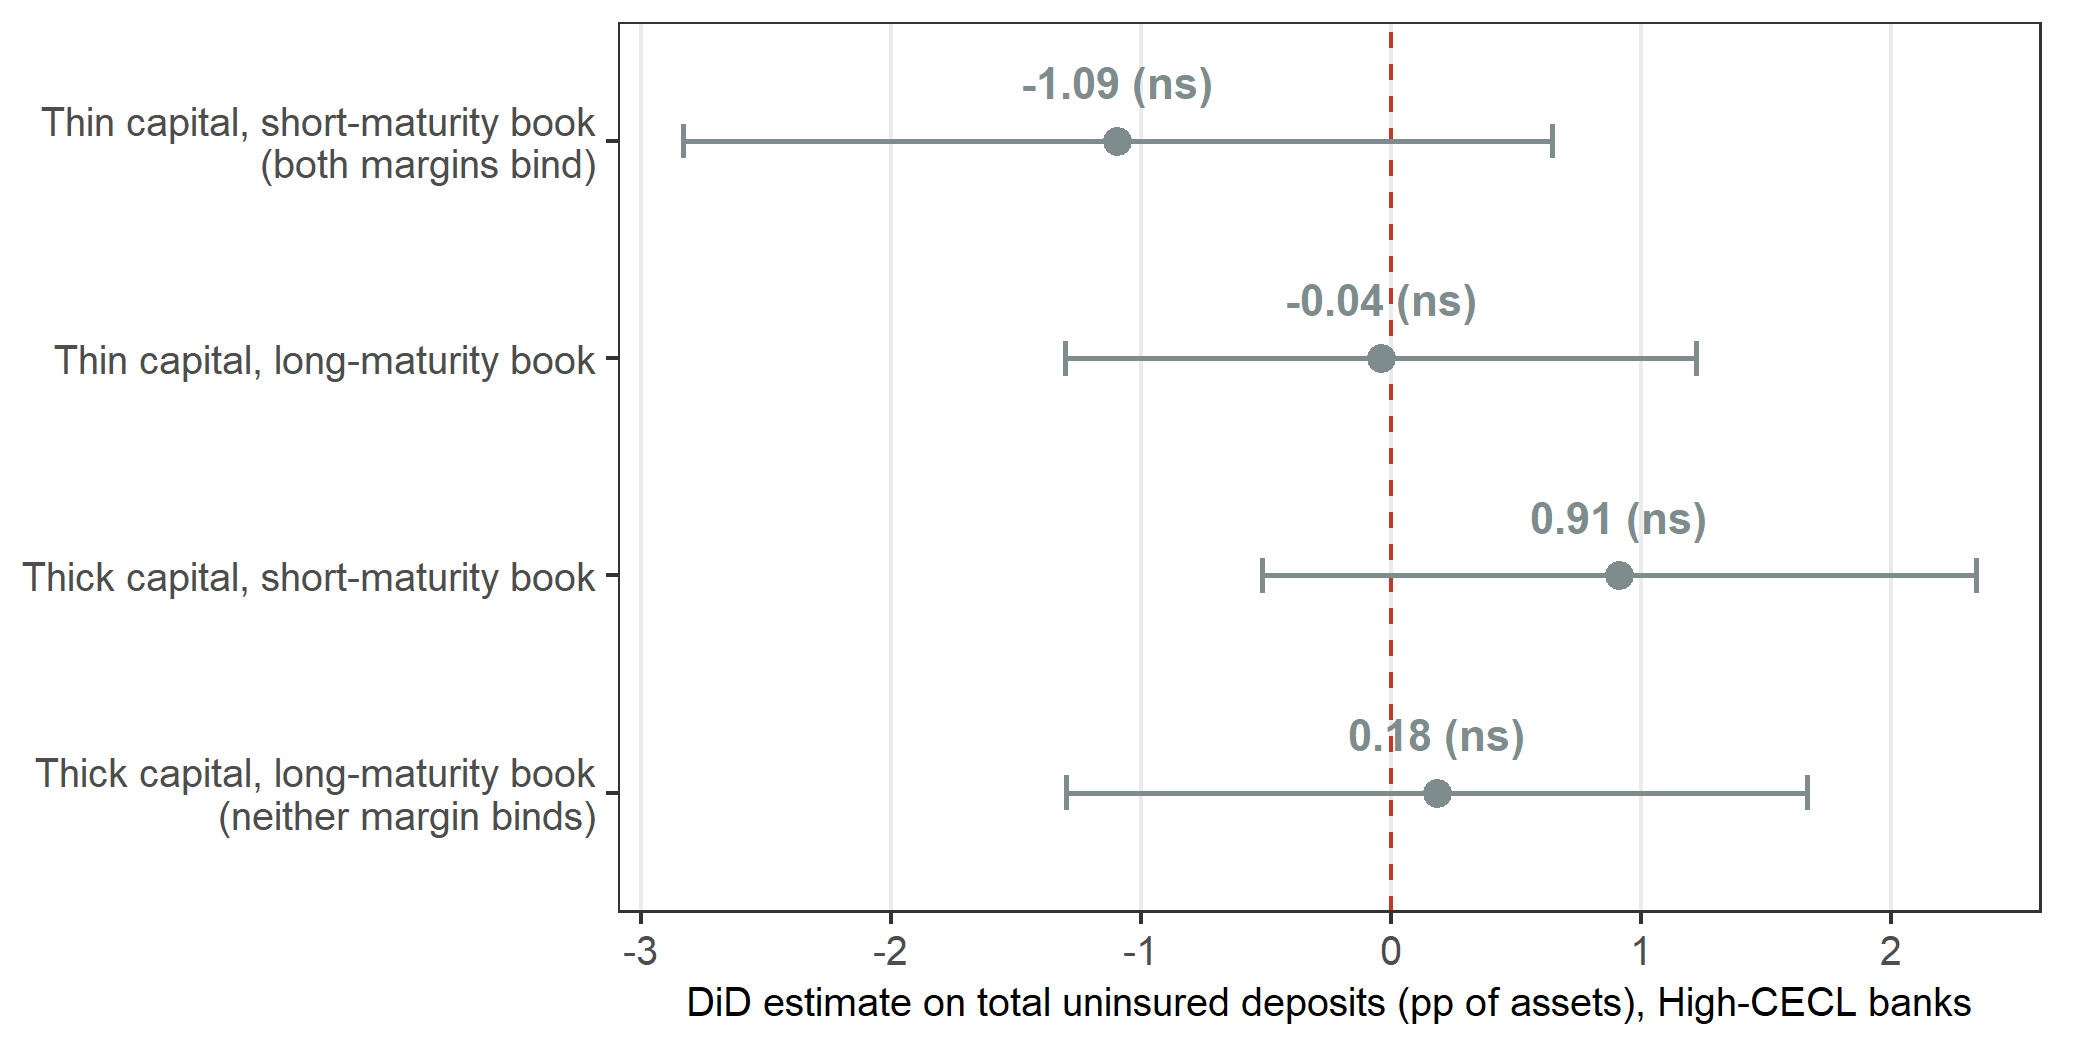
\includegraphics[width=0.76\linewidth,height=0.6\textheight,keepaspectratio]{fig_s_capital_maturity_2x2_total.png}
\end{frame}

% =============================================================================
\begin{frame}[label=frates]{High-CECL banks never defended their funding on price}
  \spec{Implied rates from Call Report interest expense; posted APYs from RateWatch, bank-week panel \quad \pill{apprates}{detail}}
  \centering
  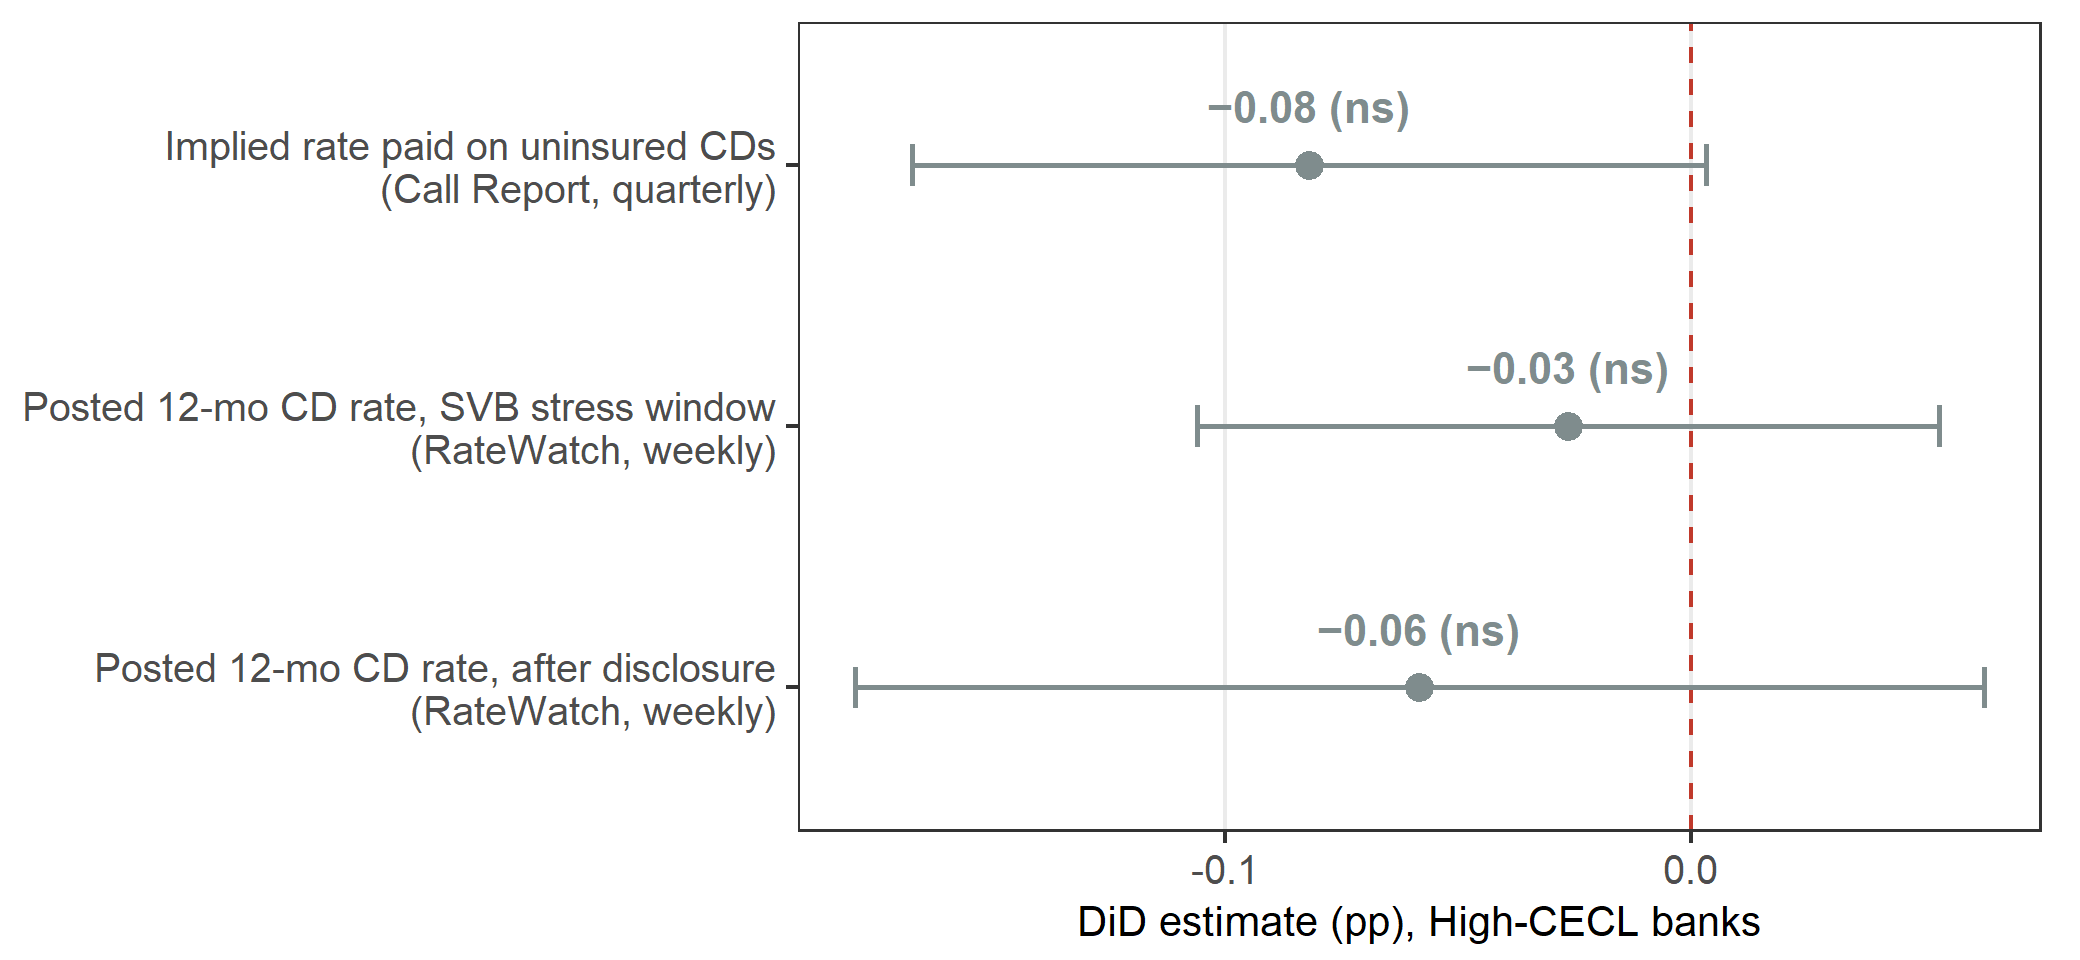
\includegraphics[width=0.8\linewidth,height=0.7\textheight,keepaspectratio]{fig_s_coef_rates.png}
\end{frame}

% =============================================================================
\begin{frame}{Where did the funding come from? Insured brokered deposits}
  \spec{DiD estimates for the three replacement margins, High-CECL banks, pp of assets}
  \begin{columns}[T]
    \begin{column}{0.55\textwidth}
      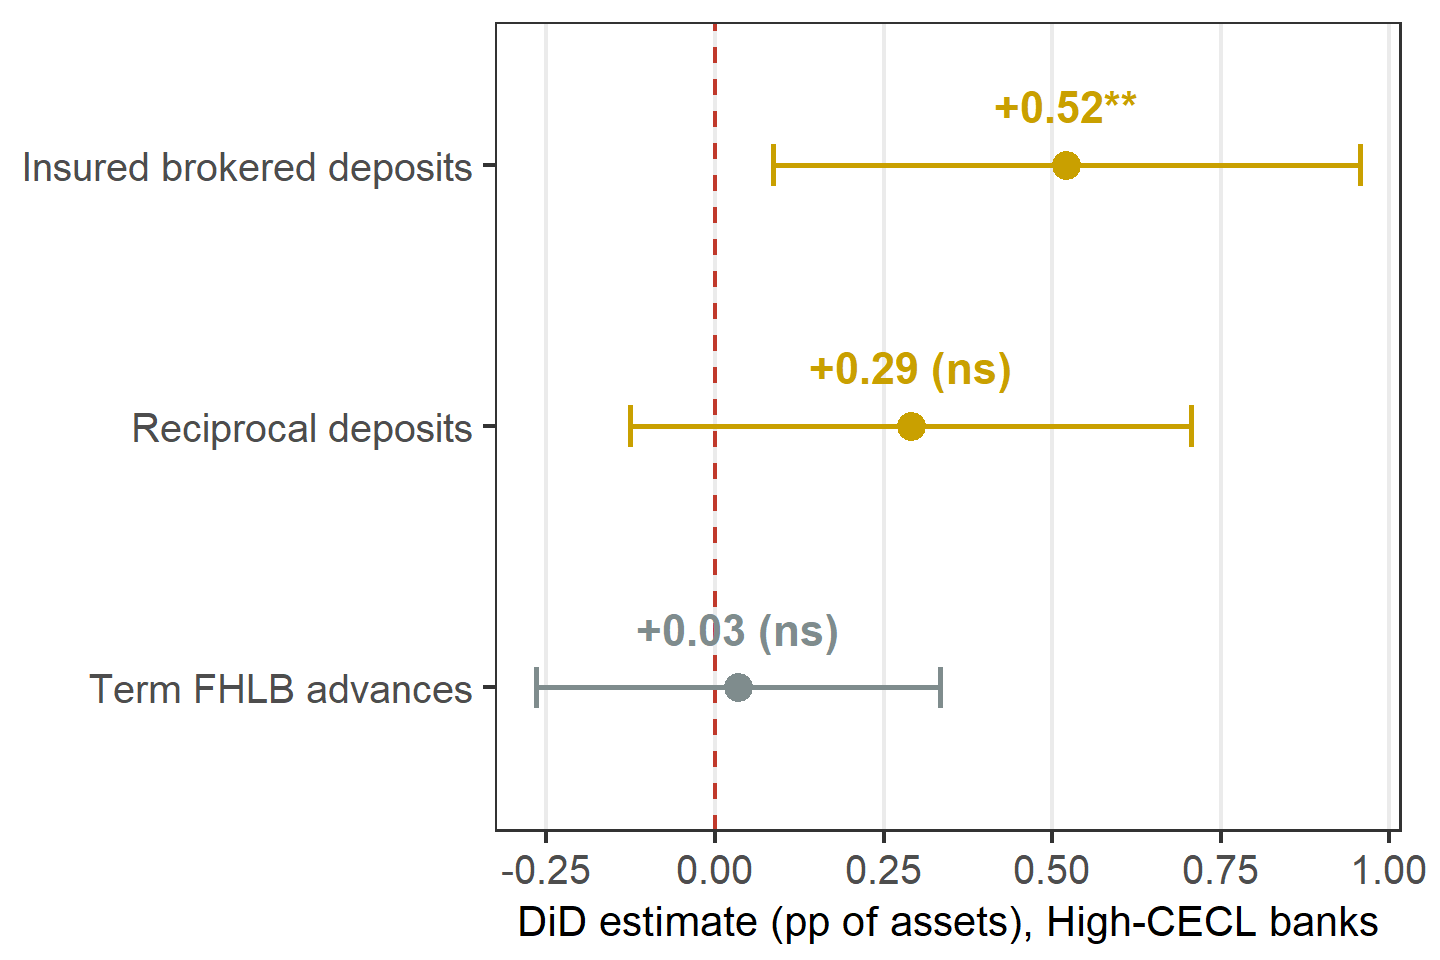
\includegraphics[width=\linewidth,height=0.72\textheight,keepaspectratio]{fig_s_coef_destination.png}
    \end{column}
    \begin{column}{0.43\textwidth}
      \begin{center}
      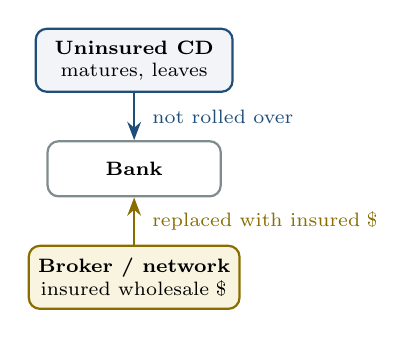
\begin{tikzpicture}[every node/.style={font=\scriptsize, align=center}]
        \node[draw=pblue, thick, rounded corners, fill=pblue!6,
              minimum width=2.5cm, minimum height=0.8cm] (dep)
              {\textbf{Uninsured CD}\\matures, leaves};
        \node[draw=pgray, thick, rounded corners, fill=white,
              minimum width=2.2cm, minimum height=0.7cm,
              below=0.6cm of dep] (bank) {\textbf{Bank}};
        \node[draw=pgolddark, thick, rounded corners, fill=pgold!12,
              minimum width=2.5cm, minimum height=0.8cm,
              below=0.6cm of bank] (brk)
              {\textbf{Broker / network}\\insured wholesale \$};
        \draw[-{Stealth}, thick, pblue] (dep) -- (bank)
          node[midway, right=1mm] {not rolled over};
        \draw[-{Stealth}, thick, pgolddark] (brk) -- (bank)
          node[midway, right=1mm] {replaced with insured \$};
      \end{tikzpicture}
      \end{center}
      \vspace{1mm}
      {\footnotesize Total funding is unchanged. What changes is the
      \emph{insurance status} of the funding. No move in uninsured
      brokered money or FHLB borrowing.}
    \end{column}
  \end{columns}
\end{frame}

% =============================================================================
\begin{frame}{Banks moved first, on private information}
  \spec{Insured brokered deposits, event study; High-CECL $\times$ event time; 90\% CI \quad \pill{appphasein}{phase-in mechanics}}
  \centering
  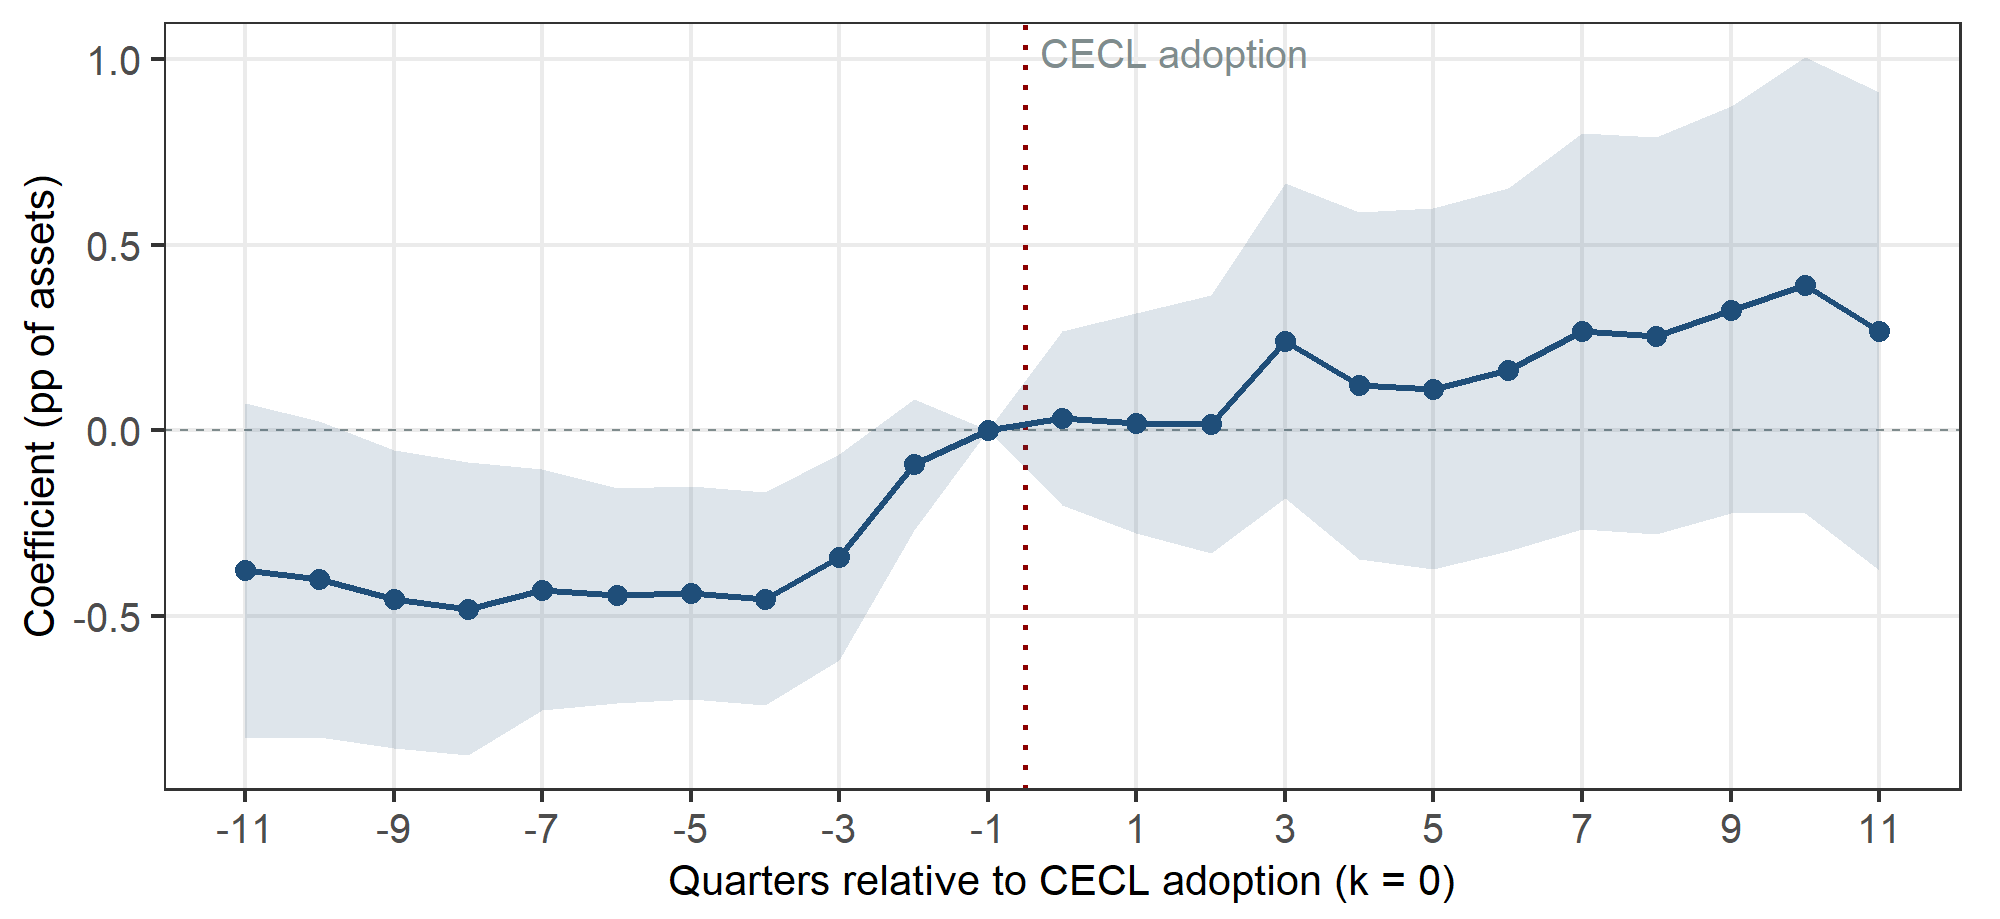
\includegraphics[width=0.9\linewidth,height=0.76\textheight,keepaspectratio]{fig_s_brokered_build1.png}
\end{frame}

\begin{frame}[label=ftiming]{Banks moved first, on private information}
  \spec{Banks ran CECL in parallel through 2022. Management knew the number before the public did}
  \begin{columns}[T]
    \begin{column}{0.63\textwidth}
      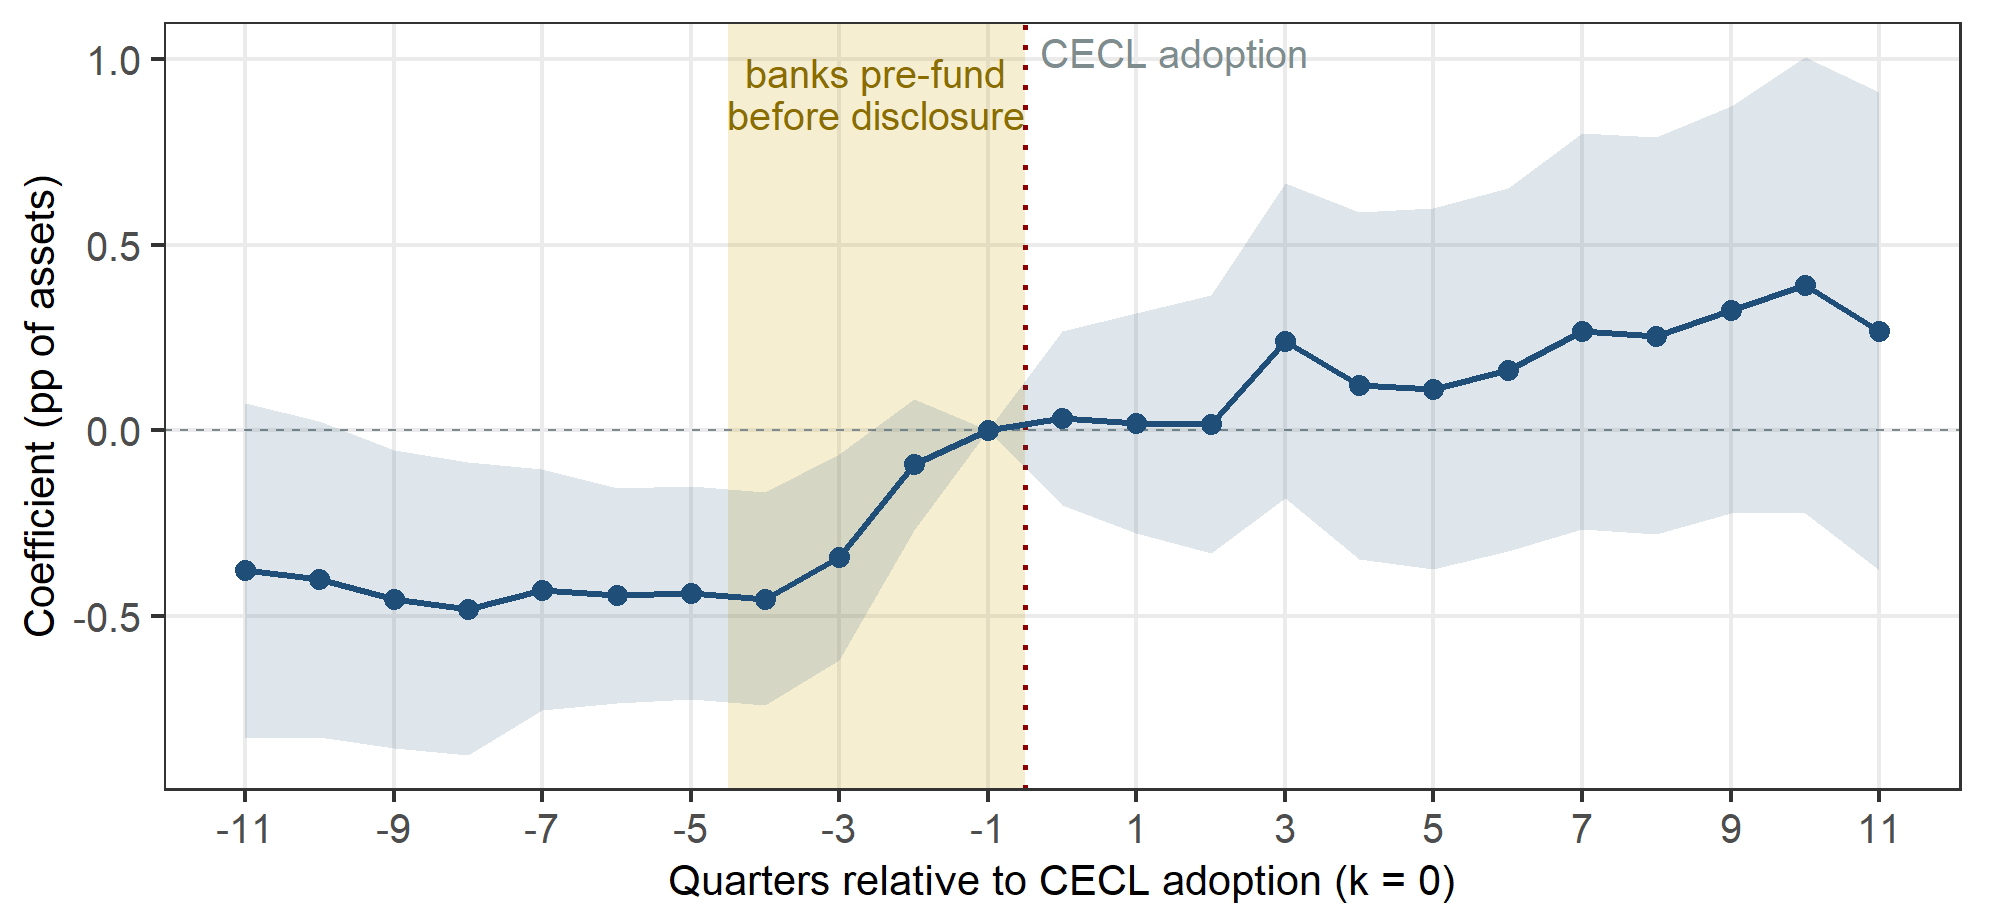
\includegraphics[width=\linewidth,height=0.6\textheight,keepaspectratio]{fig_s_brokered_build2.png}
    \end{column}
    \begin{column}{0.35\textwidth}
      {\scriptsize
      \textbf{The ramp scales with the still-undisclosed charge.}\\[0.5mm]
      $\Delta$ insured brokered/assets, $k=-4$ to $-1$, on the charge
      disclosed at $k=0$:\\
      \hspace*{2mm}$+$0.13*** pp per pp of charge\\
      \hspace*{2mm}$+$0.53*** pp for High-CECL banks\\[0.8mm]
      \textbf{And does not vary by capital or maturity.} Interactions with
      2022Q4 capital and CD maturity all insignificant. The depositor response
      sits in one cell; the bank response does not.\\[0.8mm]
      Phase-in electors pre-funded 0.41** pp more.
      \pill{appphasein}{detail} \pill{appretention}{who kept it}}
    \end{column}
  \end{columns}
  \vspace{-1mm}
  \takeaway{Bank margins move on private information, before adoption;
    depositor margins move only when the number becomes public}
\end{frame}

% =============================================================================
\begin{frame}{The substitution is costly: funding costs up, profitability down}
  \spec{Event studies for interest expense, ROA, NIM; High-CECL $\times$ event time; 90\% CI}
  \begin{columns}[T]
    \begin{column}{0.33\textwidth}
      \centering {\small Interest expense\ \textcolor{pred}{$\uparrow$ 8--9bp/yr}}\\
      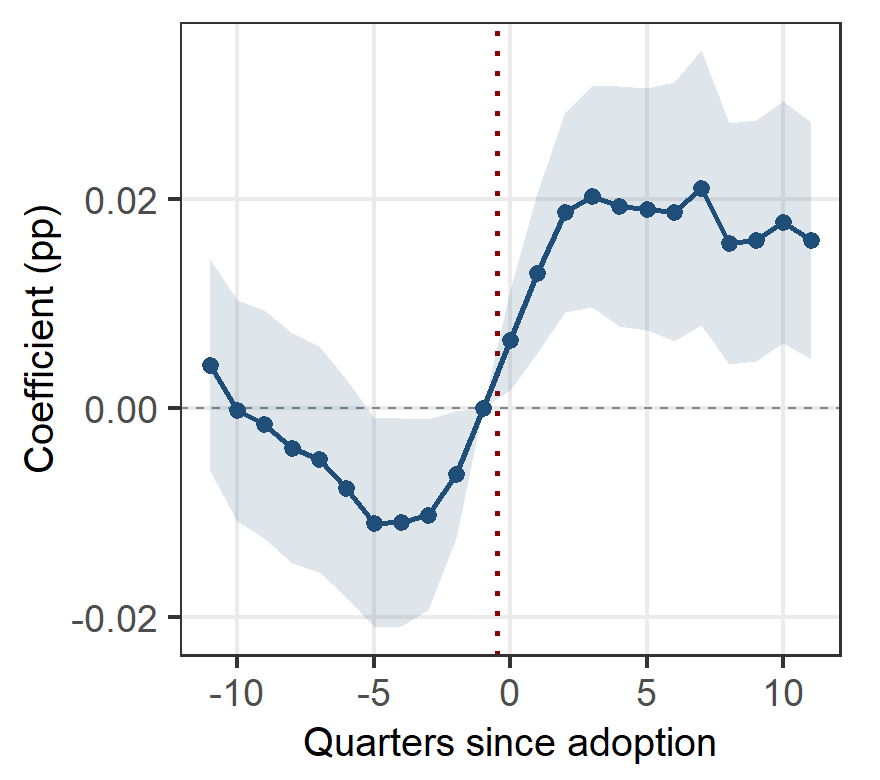
\includegraphics[width=\linewidth,height=0.56\textheight,keepaspectratio]{fig_s_es_intexp.png}
    \end{column}
    \begin{column}{0.33\textwidth}
      \centering {\small ROA\ \textcolor{pred}{$\downarrow$ 15bp/yr}}\\
      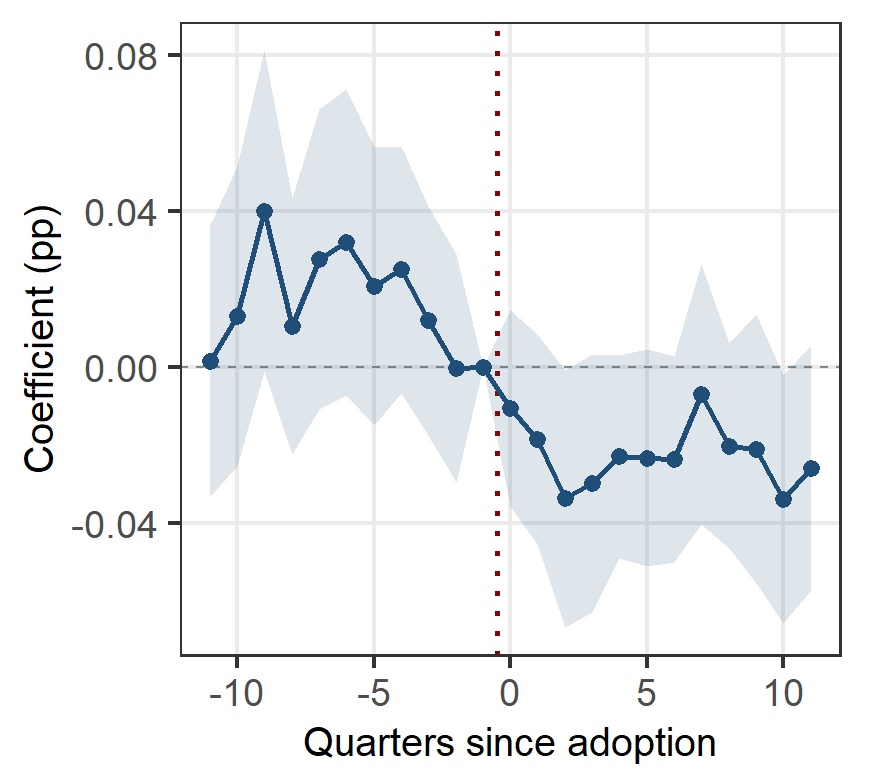
\includegraphics[width=\linewidth,height=0.56\textheight,keepaspectratio]{fig_s_es_roa.png}
    \end{column}
    \begin{column}{0.33\textwidth}
      \centering {\small NIM\ \textcolor{pred}{$\downarrow$ 9bp/yr}}\\
      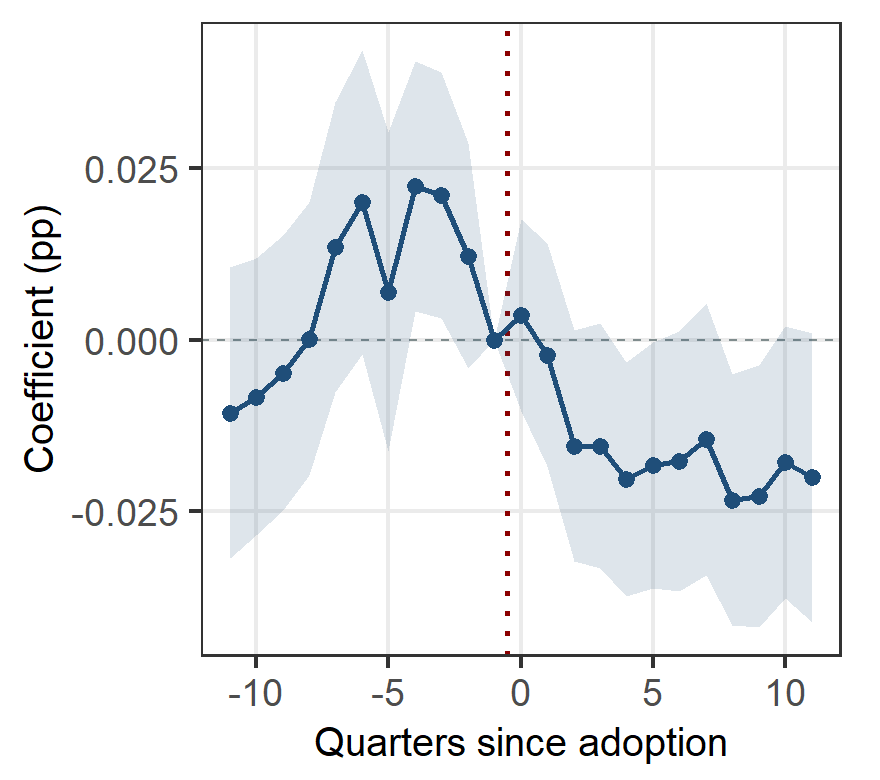
\includegraphics[width=\linewidth,height=0.56\textheight,keepaspectratio]{fig_s_es_nim.png}
    \end{column}
  \end{columns}
  \vspace{-1mm}
  \takeaway{No premium to stayers, no higher posted rates. The cost comes from
    replacing maturing uninsured CDs with insured wholesale money raised at
    wholesale rates}
\end{frame}

% =============================================================================
\begin{frame}{Is this the SVB stress in disguise?}
  \spec{CECL disclosures reached the public in April--May 2023, weeks after the March 2023 failures}
  \begin{itemize}
    \item The concern: uninsured depositors were already running from
      vulnerable banks. The CECL charge may simply proxy for that
      vulnerability
    \item 2023 runs were wholesale, at public banks; this sample is private
      and retail-funded \gcite{Cipriani--Eisenbach--Kovner '24}
    \pause
    \item Three tests:
      \begin{itemize}
        \item[1.] \textbf{Placebo.} Banks with no CECL news, sorted on run
          exposure: do their uninsured CDs separate after March 2023?
        \item[2.] \textbf{Orthogonality.} Is the charge correlated with
          unrealized losses, asset maturity, or uninsured funding?
        \item[3.] \textbf{Horse race.} Do the CECL estimates survive
          controlling for stress exposure directly?
      \end{itemize}
  \end{itemize}
\end{frame}

% =============================================================================
\begin{frame}{Placebo: zero-charge banks split by 2022Q4 unrealized losses}
  \spec{Zero-charge banks split at the median 2022Q4 unrealized loss; group means, no controls or FE \quad \pill{appplacebo}{placebo detail}}
  \centering
  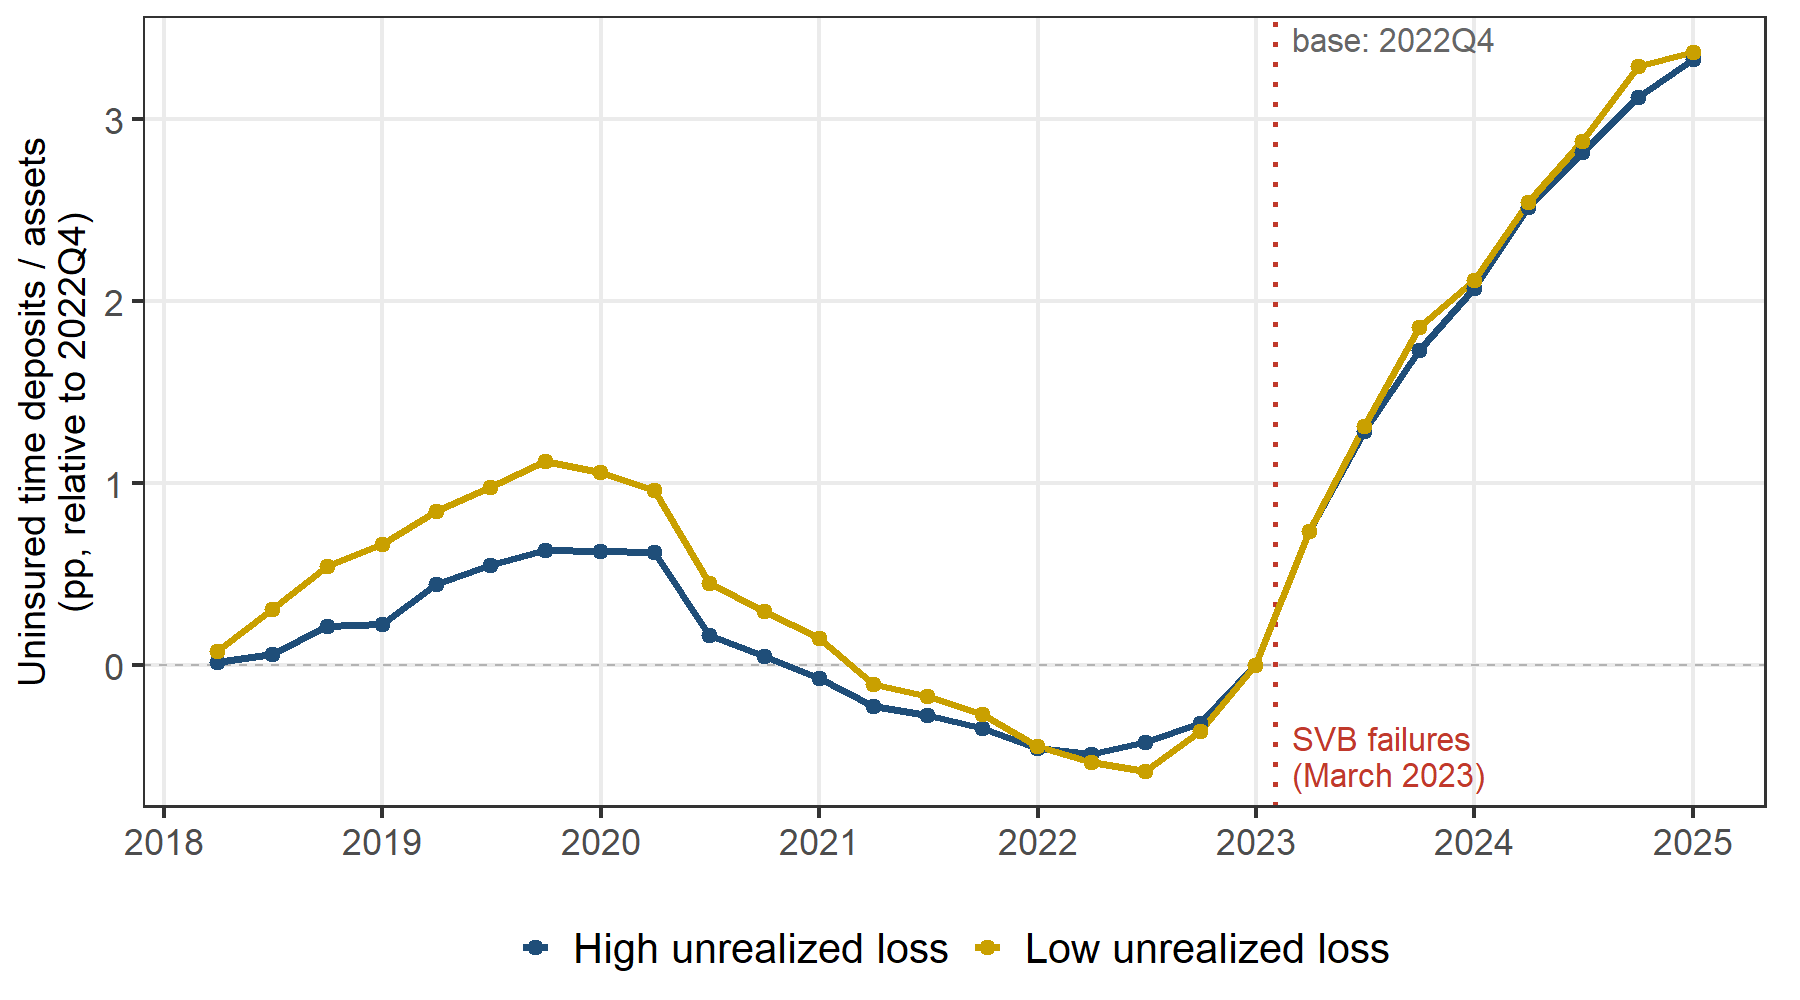
\includegraphics[width=\linewidth,height=0.7\textheight,keepaspectratio]{fig_s_placebo_svb.png}
  \vspace{-1mm}
  \takeaway{Banks with no CECL news show no separation on run exposure}
\end{frame}

% =============================================================================
\begin{frame}[label=fsvb]{Treatment is orthogonal to run exposure}
  \spec{2022Q4 stress-vulnerability characteristics across deciles of the disclosed charge (positive-adjustment banks) \quad \pill{appplacebo}{placebo detail}}
  \begin{columns}[T]
    \begin{column}{0.58\textwidth}
      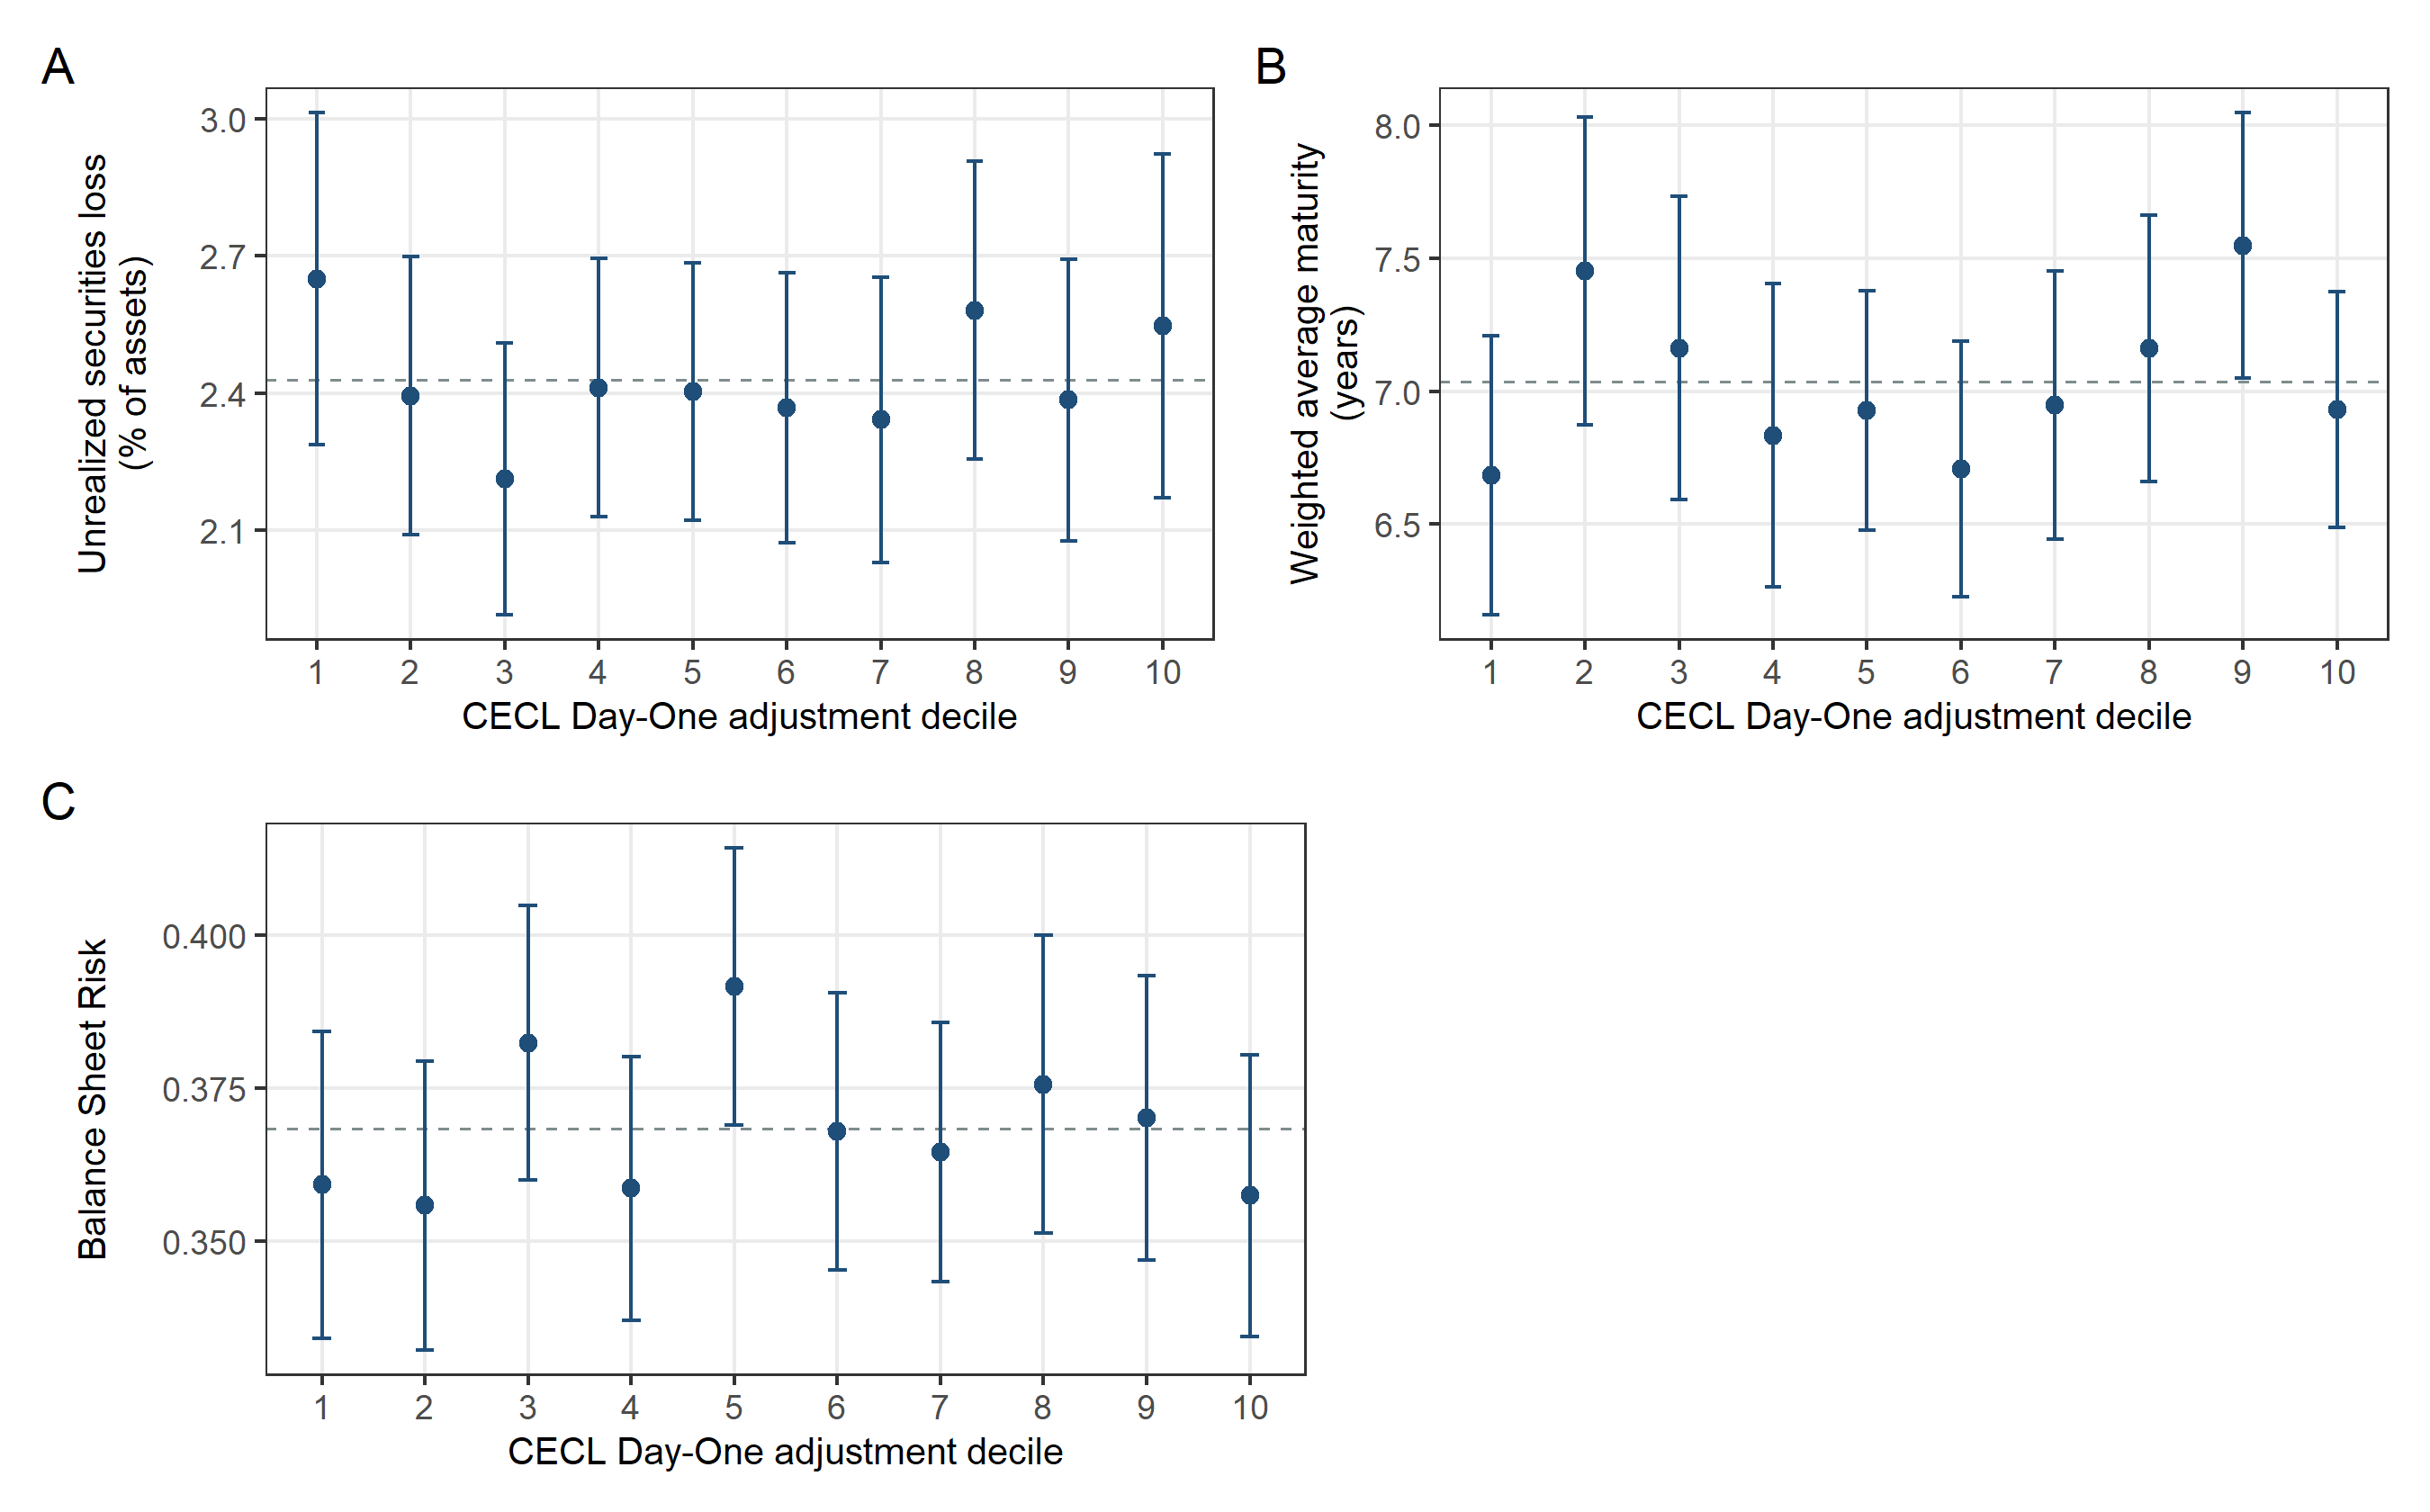
\includegraphics[width=\linewidth,height=0.76\textheight,keepaspectratio]{fig_svb_exposure_20260811.png}
    \end{column}
    \begin{column}{0.4\textwidth}
      \footnotesize
      \begin{itemize}
        \item Treatment $\perp$ run exposure: unrealized losses, asset
          maturity, Balance Sheet Risk
          \gcite{Huberdeau-Reid--Pennacchi '25} all flat; $<$1\% of
          variation explained
        \item Horse race: CECL estimates unchanged
      \end{itemize}
    \end{column}
  \end{columns}
\end{frame}

% =============================================================================
\begin{frame}{What I cannot rule out: attention}
  \spec{The design identifies the response to the disclosure, conditional on the level of depositor attention in 2023}
  \begin{itemize}
    \item Treatment is not stress exposure. But 2023 was a year of unusual
      attention to bank fragility
    \item After March 2023, depositors may have paid closer attention to
      any bad news about their bank
    \item If so, the estimates are an upper bound on what the same number
      would do in a quiet year
    \item Banks pre-funded in 2022, before SVB, in proportion to their charge.
      They expected depositors to react before there was any run to watch
  \end{itemize}
\end{frame}

% =============================================================================
\begin{frame}{Takeaways}
  \spec{A mandatory credit-risk disclosure moved uninsured funding at solvent community banks}
  \begin{enumerate}
    \item<1-> \textbf{Uninsured depositors respond to the disclosure.} Uninsured CDs fell
      and insured CDs rose in proportion to the disclosed charge. Flat for
      five years before, breaking only at public disclosure
    \item<1-> \textbf{Discipline = quantity exit at the rollover margin.} No
      repricing, no move in operating balances, stronger where more CDs came
      due and where capital buffers were thin
    \item<1-> \textbf{Banks repurchased the insurance.} Insured brokered
      money replaced monitored money; interest expense rose and profitability
      fell. Discipline shows up as a higher cost of funding
    \item<1-> \textbf{Private coverage may already be dampening discipline.}
      Reciprocal networks, sweeps and insured brokered CDs convert uninsured
      balances into insured ones with no change in the balance sheet
  \end{enumerate}
  \vfill
  \begin{center}
    \textcolor{pgray}{\small dimuthu.ratnadiwakara@rich.frb.org}
  \end{center}
\end{frame}

% =============================================================================
\appendix

\begin{frame}[label=apppredictors]{Backup: the charge is hard to predict}
  \spec{Cross-section of the Day-One charge on 2022Q4 observables}
  \begin{itemize}
    \item Loads modestly on NPL ratio, size, capital, deteriorating ROA trend
      in directions consistent with credit-sensitive books needing larger
      lifetime reserves
    \item Adjusted $R^2 \approx 1.4\%$ in the most saturated specification
      (fundamentals + deposit mix + performance trends + local market HHI)
    \item High-CECL banks are \emph{not} observably weak banks relabeled:
      almost all variation is orthogonal to anything a depositor could see
      before disclosure
  \end{itemize}
  \hfill \pill{ftreat}{back}
\end{frame}

\begin{frame}[label=apprates]{Backup: rate tests in detail}
  \spec{Implied rates: Call Report interest expense on time deposits above/below \$250k (2017--)}
  \begin{itemize}
    \item Implied rate on uninsured CDs, Post $\times$ High-CECL: $-0.082$
      (SE 0.052). No premium extracted by depositors who stayed
    \item Within-bank large--small rate spread: $-0.110^{*}$; if anything
      narrows
    \item RateWatch posted APYs (weekly, $\sim$3{,}300 banks): 12-mo CD
      \$10k/\$100k tiers and savings, no differential move in stress window
      ($-0.026$, SE 0.048) or post-publication ($-0.058$, SE 0.074)
    \item $>$90\% of branches follow centrally set rates
      \gcite{Begenau--Stafford '23}; healthy banks can bid for uninsured
      money, weak banks cannot \gcite{Maechler--McDill '06}
  \end{itemize}
  \hfill \pill{frates}{back}
\end{frame}

\begin{frame}[label=appphasein]{Backup: the capital phase-in election}
  \spec{Call Report Schedule RC-R Part I item 2.a; elected on the first CECL filing, irrevocable}
  \begin{itemize}
    \item Election spreads the Day-One hit to \emph{regulatory} capital over
      three years: 75\% added back in year one, 50\%, 25\%, full impact from
      year four
    \item Economically sensible only if the bank expects a material hit;
      election probability rises 0.072*** per pp of charge
    \item 34\% of High-CECL banks elect vs.\ 6\% of the rest; electors'
      pre-adoption insured-brokered ramp is 0.41** pp larger
    \item Election is measured \emph{at} the first CECL filing; only the
      brokered ramp is genuinely quarters early
  \end{itemize}
  \hfill \pill{ftiming}{back}
\end{frame}

\begin{frame}[label=appretention]{Backup: who kept the brokered money?}
  \spec{High-CECL banks that pre-funded (insured brokered ramp $>0$, $k=-4$ to $-1$), split at the median post-adoption change in uninsured CDs ($k=-1$ to $+8$); pp of assets, winsorized 1/99}
  \begin{center}
  \footnotesize
  \setlength{\tabcolsep}{6pt}
  \renewcommand{\arraystretch}{1.25}
  \begin{tabular}{lcccc}
    \toprule
    & N & Pre-adoption ramp & Post $\Delta$ brokered & $\Delta$ unins.\ CDs \\
    \midrule
    Uninsured CDs grew least & 44 & $+$4.16 & $+$2.46 & $+$0.53 \\
    Uninsured CDs grew normally & 16 & $+$2.95 & $-$1.22 & $+$5.05 \\
    \midrule
    Difference in $\Delta$ brokered & & & $+$4.33*** (1.34) & \\
    \bottomrule
  \end{tabular}
  \end{center}
  \begin{itemize}\footnotesize
    \item Both groups bought 3--4 pp of insured brokered money before the number was public
    \item Where uninsured CDs then failed to grow, the brokered money stayed and grew;
      where they grew normally, it ran off
    \item Difference controls for ramp size, log assets, equity/assets (robust SE)
  \end{itemize}
  {\scriptsize Descriptive: 16 banks in the second row; split is on a
  post-adoption outcome. Uninsured CDs rose at almost every bank in 2023--25, so
  ``grew least'' is relative, not a net outflow.} \hfill \pill{ftiming}{back}
\end{frame}

\begin{frame}[label=appcapital]{Backup: capital-buffer interaction, full specification}
  \spec{Moderator: equity/assets frozen at 2022Q4, winsorized 1/99; gap outcome = uninsured $-$ insured time deposits/assets}
  \begin{itemize}
    \item Post $\times$ CECL Adj $\times$ Equity$_{22Q4}$: $+0.0665^{***}$
      (0.019); binary analog $+0.31^{***}$
    \item Main effect at zero equity: $-0.80^{***}$ (continuous),
      $-4.12^{***}$ (binary)
    \item Level-outcome analog: $+0.0275^{**}$; robust to dropping the
      time-varying equity control
    \item Implied effect crosses zero at equity $\approx$ 12--13\%, just above
      the 75th percentile; best-capitalized quartile shows essentially no
      response
  \end{itemize}
  \hfill \pill{fcapital}{back}
\end{frame}

\begin{frame}[label=appplacebo]{Backup: SVB placebo and horse race}
  \spec{DiD around March 2023 with 2022Q4 unrealized securities loss as intensity}
  \begin{itemize}
    \item Zero-charge banks ($\sim$2{,}278, no CECL news): Post-SVB $\times$
      loss $= +0.073^{**}$ for uninsured CDs, the \emph{wrong sign} for a run;
      insured CDs move the same way ($+0.062^{*}$) $\Rightarrow$ rate-cycle
      funding mix, not flight
    \item Full-sample horse race: CECL coefficients essentially unchanged
      ($-0.078^{**}$ continuous, $-0.406^{**}$ High-CECL); loss interaction
      small and insignificant
    \item Uninsured deposit share enters the charge cross-section
      \emph{negatively} ($-0.003^{**}$): high-CECL banks held slightly fewer
      of the deposits that ran in 2023
  \end{itemize}
  \hfill \pill{fsvb}{back}
\end{frame}

\begin{frame}[label=appes]{Backup: five-year pre-period, balanced endpoints}
  \spec{Extended event studies from 2018Q1; edge bins pool $k\leq-20$ and $k\geq+11$; joint pre-trend tests}
  \begin{columns}[T]
    \begin{column}{0.5\textwidth}
      \centering {\small Uninsured time deposits \quad ($p=0.18$)}\\
      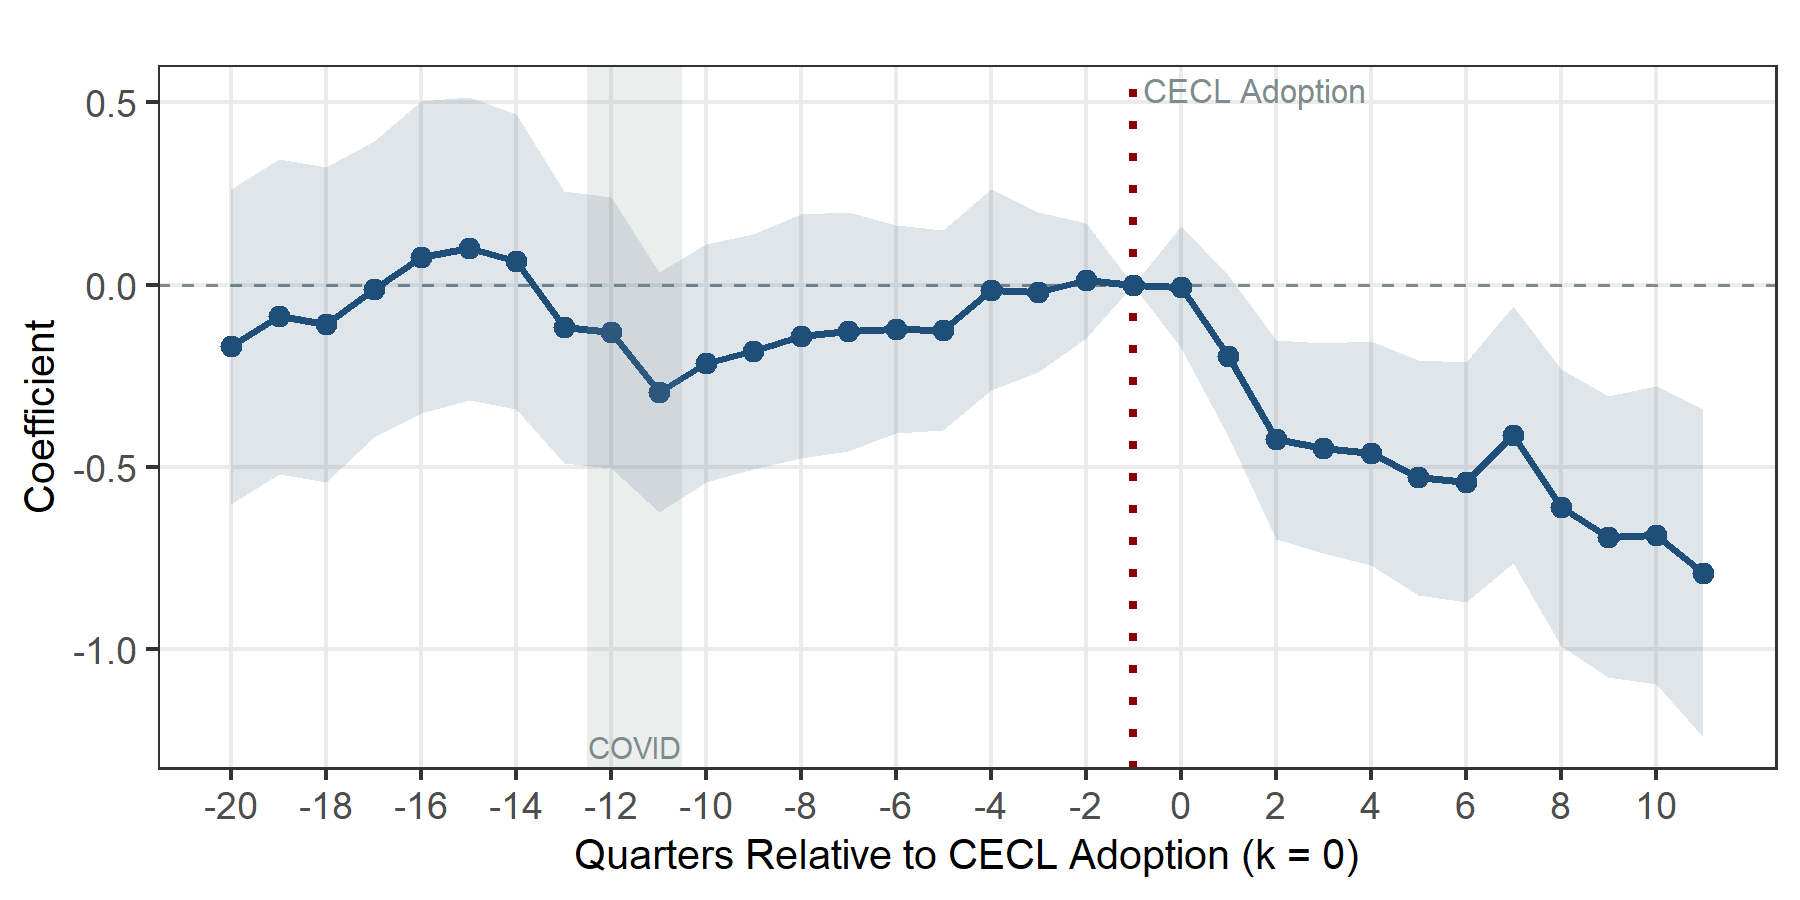
\includegraphics[width=\linewidth]{fig_es_long_unins_balanced_20260806.png}
    \end{column}
    \begin{column}{0.5\textwidth}
      \centering {\small Insured time deposits \quad ($p=0.37$)}\\
      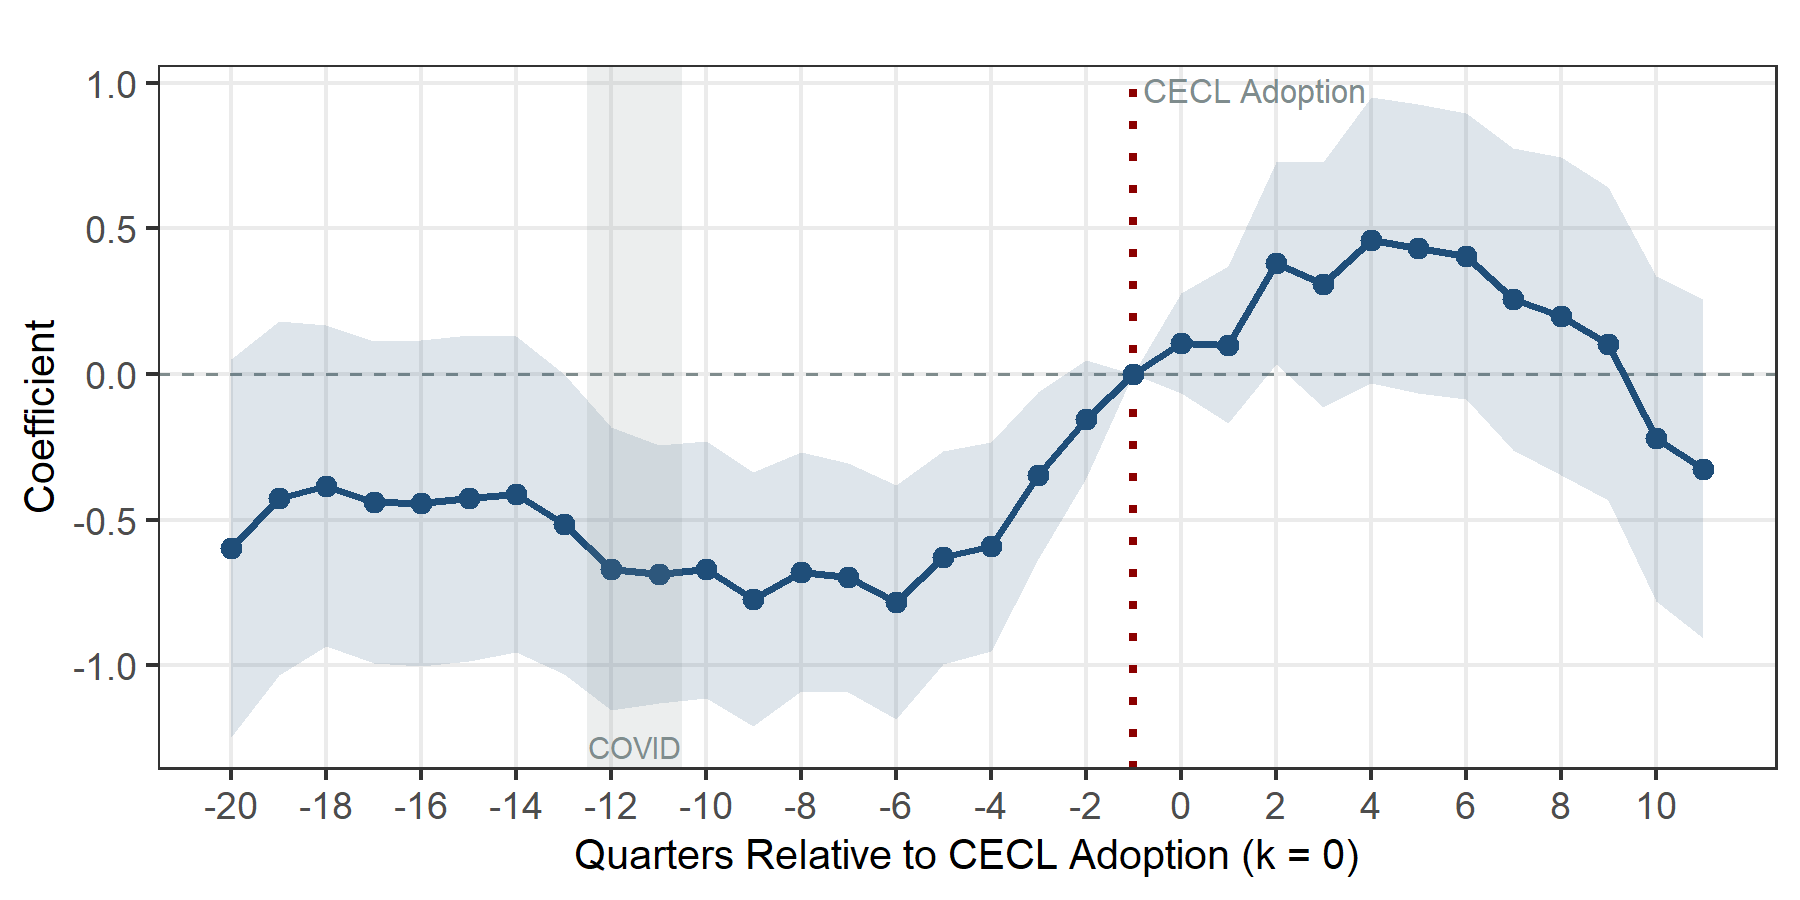
\includegraphics[width=\linewidth]{fig_es_long_ins_balanced_20260806.png}
    \end{column}
  \end{columns}
  \vspace{2mm}
  {\footnotesize Late upward drift in the insured series is the banks' own
  pre-funding footprint (insured brokered CDs are booked as time deposits);
  absorbed into the $k=-1$ baseline, so post coefficients \emph{understate}
  the total movement.}
\end{frame}

\end{document}
